\chapter{Cretaceous origin of viral domestication in Eucoilini parasitoids}
\label{chap:Papier3_datation}

\begin{center}
        \Large Benjamin Guinet$^{\text{1}}$, Jonathan Vogel $^{\text{2}}$, Ralph Peters  $^{\text{2}}$, Jan Hrcek $^{\text{3}}$, Matthew L. Buffington$^{\text{4}}$, Julien Varaldi $^{\text{1}}$\\
        \vspace{0.5cm}
        \normalsize
        $^{\text{1}}${Université Lyon 1, CNRS, Laboratoire de Biométrie et Biologie Evolutive UMR 5558, F-69622 Villeurbanne, France.}\\
        $^{\text{2}}${Zoologisches Forschungsmuseum Alexander Koenig Adenauerallee 16053113 Bonn, Germany.}\\
        $^{\text{3}}${Biology Centre of the Czech Academy of Sciences Branišovská 1160/31, 370 05 České Budějovice, Czech Republic.}\\
        $^{\text{4}}${USDA-ARS Systematic Entomology Laboratory, Washington D.C., USA.}\\
\end{center}
\setcounter{minitocdepth}{1}
{\hypersetup{linkcolor=GREYDARK}\minitoc}

\label{sec:chap3}
\newpage

\section{Reproducibility and Supplemental material}

All supplementary material named with a "GitHub" mark, can be found within the following GitHub repository : \href{https://github.com/BenjaminGuinet/PhD_defense/tree/main/Supplementary_paper3}{Supplementary\_paper3}. An e-mail authorization must have been sent to all members of the jury. 


\section{Abstract}
    
In addition to symbiotic bacteria, insects are frequently associated with viruses that can influence their phenotypes. The association between the dsDNA virus LbFV and the endoparasitoid wasp \textit{Leptopilina boulardi} is an exceptional example of their contribution to insect phenotype. These wasps lay their eggs in \textit{Drosophila} larvae, and the development of their offspring ultimately results in the larvae's death. By inducing superparasitism, the heritable virus LbFV manipulates the oviposition behaviour of these wasps (laying eggs in already parasitized hosts). This alteration in behaviour favours the horizontal transmission of the virus within superparasitized hosts, thereby facilitating the virus' efficient spread among wasp populations. This virus belongs to the newly described Filamentoviridae virus family. Intriguingly, genomic analyses of several parasitoid species (including \textit{Leptopilina sp.}) revealed the presence of multiple genes of viral origin deriving from a massive horizontal transfer involving a LbFV-like virus that occurred in the distant past. These viral sequences have been domesticated by parasitic wasps and enable the delivery of immunosuppressive factors into host immune cells, thereby protecting parasitoid progeny from the host immune response. In this study, we provide evidence that the majority of parasitoid species belonging to the Eucoilini tribe (Cynipoidea, Figitidae) are concerned by this endogenization event which occurred 75 million years ago, coinciding with the radiation of their Schizophora hosts. In addition, we describe a second, more recent independent event within one of the Eucoilini species, in which at least one gene likely replaced the function of a previous filamentous EVE inherited from the first ancestral event. Finally, using the new event to calibrate the virus phylogeny, we suggest that Filamentoviridae and Hymenoptera have co-existed for a long period of time, indicating a deep-rooted relationship between filamentous viruses and their Hymenoptera hosts.

\section{Introduction}

Horizontal gene transfer (HGT) can be defined as the acquisition of genetic material from unrelated organism. HGT may involve viruses as donors, and in some cases entire viral genomes can integrate into their hosts' chromosomes. Integrated part of viral genomes are called as Endogenous viral Elements (EVEs). Several examples suggest that EVEs have enabled major genetic innovations in eukaryotes. Such elements are called domesticated endogenous viral elements (dEVEs) \citep{gasmi_horizontally_2021,yan_origin_2009,suzuki_non-retroviral_2020,parker_laterally_2019}. One of the most sophisticated examples of viral domestication concerns endoparasitoid wasps. Endoparasitic wasps lay their eggs within the bodies of other arthropods (usually eggs or larval stages), ultimately killing them in the process. During the interaction, parasitoid offspring is exposed to the host's immune system. Those wasps have repeatedly domesticated not only single genes, but entire viral machineries \citep{burke_common_2019}. Notably, the ancestor of at least five monophyletic clades of endoparasitic wasps each domesticated a battery of viral genes allowing them to construct a vector toolkit delivering DNA encoding immunosuppressive factors or immunosuppressive proteins {\citep{bezier_polydnaviruses_2009,volkoff_analysis_2010,pichon_recurrent_2015,burke_common_2019,di_giovanni_behavior-manipulating_2020}}. When DNA is transferred into the host (so-called polydnaviruses, PDVs), it integrates into the host hemocyte's DNA and is expressed \citep{chevignon_functional_2014, muller_genome-wide_2021}, influencing the host's physiology and behaviour and ultimately favoring the development of wasp offspring. In instances where proteins are transmitted (so-called virus-like particles, VLPs), the viral machinery enables the distribution of these virulence proteins into host immune cells, hence suppressing the host immune response \citep{colinet_convergent_2007}.\\ 

The most recent case documented involves the domestication of 13 EVEs deriving from the Leptopilina boulardi filamentous virus (LbFV). These virally-derived genes are involved in the synthesis of VLPs in multiple species of the \textit{Leptopilina} genus \cite{di_giovanni_behavior-manipulating_2020}.
LbFV is part of a recently proposed family of large double-stranded DNA viruses discovered in multiple endoparasitoid species (\hyperref[sec:chap2]{chapitre 2}:\textit{in prep}) (the Filamentoviridae). Interestingly, in that system, the free-living infectious virus LbFV is still infecting one of the species of the clade. LbFV is transmitted vertically among \textit{Leptopilina boulardi} wasps in which it affects the wasp egg-laying behavior: infected females readily accept to lay their eggs in already parasitized hosts, contrary to uninfected ones \citep{varaldi_artifical_2006,varaldi_infectious_2003}. This induction of "superparasitism" permits virus horizontal transmission in superparasitism, thus increasing its fitness at the expense of wasp fitness \citep{gandon_superparasitism_2006}. The 13 domesticated LbFV-like EVEs are found in the three \textit{Leptopilina} species tested so far and their distributions in their genomes comprise several syntenic blocks suggesting a common origin for all these genes (Di Giovanni et al., 2020). In addition, the EVE phylogenies are identical to the wasp phylogeny, further validating this hypothesis of a single ancestral origin (Di Giovanni et al., 2020). These EVEs are specifically expressed in the venom gland during the early pupal stage of the wasp, when VLPs are being synthesized. In that system, a viral DNA polymerase (ORF58) allows the amplification of a portion of the EVEs (10/13) and thus increases their expression profile (Di Giovanni et al., 2020). Those genes are probably involved in transcription (\textit{lef-4}, \textit{lef-8}, and \textit{lef-9}), DNA replication (\textit{DNApol}, \textit{helicase}), virulence protein wrapping (\textit{ac81}), and lipid membrane formation (\textit{lcat}) (Di Giovanni et al., 2020). As would be expected for genes involved in the production of fitness-related structures like VLPs, all 13 EVEs have an intact open reading frame and are subject to strong purifying selection (\textit{\textit{dN/dS}} $<$ 1). In addition, one of these EVEs (LbFVORF85) was found as a protein in purified VLPs (Di Giovanni et al., 2020), further suggesting that the 13 EVEs play a key role in VLPs production. Other putative LbFV-related EVEs have been found in other endoparasitoid species, such as in \textit{Dolichomitus sp} (Ichneumonidae) \citep{burke_presence_2021} and \textit{Platygaster orseoliae} (\hyperref[sec:chap1]{chapitre 1}:\textit{in review}) (Platygastroidea). These species belong to other superfamilies and are thus too distant from \textit{Leptopilina} species to be part of the same endogenization event.\newline 

To date, all members of the \textit{Leptopilina} genus (6 examined) have been tested positive for the presence of one or more of these EVEs. On the contrary, the two species examined in the \textit{Ganaspis} genus (Ganaspini tribe) were negative (Di Giovanni et al., 2020). 
 This observation suggests that the endogenization event occurred after the divergence between \textit{Ganaspis} and \textit{Leptopilina} species and before the diversification of the \textit{Leptopilina} genus. However, it cannot be excluded at this stage that domestication is even older (before the divergence of Eucoilini and Ganaspini), with a secondary loss in the genus \textit{Ganaspis}. Additionally, several clades branching "between" \textit{Leptopilina} and \textit{Ganapsis} have not been analyzed yet \citep{blaimer_comprehensive_2020}. We therefore lack details about the range of species concerned by this event, as well as the long-term evolutionary history of the donor virus and its putative role in shaping the evolution of many Figitidae wasp species. \newline 

To clarify this, we looked for the presence of the filamentous-like EVEs in 26 Figitidae species. The results showed that an ancestral endogenization event involving a close relative of LhFV occurred in the common ancestor of 4 different Eucoilini genus and would have taken place in the late Cretaceous about 76.4 million years ago, well before the divergence of \textit{Leptopilina} species estimated around 40mya \citep{blaimer_comprehensive_2020}. In addition, we also point out a second independent endogenization event involving a closely relatives of LbFV that occured recently within the genome of the \textit{Rhoptromeris} species. Interstingly, this last event probably led to the replacement of one gene brought from the first ancestral event.  In light of the novel description of the putative Filamentoviridae family from which the donor virus originated, this work provides unique information on the interactions between these viruses and the wasps. It also gave us the opportunity to compare the gene content observed in filamentous viruses and in the 18 EVEs (including five additional EVEs discovered in this study) which further supported traditional views in which core genes are involved in viral-like structure production (ref Drezen). Finally, these EVEs constitute living fossil records that have been segregating in wasp populations since their endogenization. Since these EVEs are also related to contemporary viral sequences, we also used this dataset to calibrate the viral phylogeny using fossil records from wasp lineages. Through the use of this calibration, we inferred the divergence period of the entire filamentous new viral family as being around 297 millions of years ago, giving new insight into past viral activity of the Filamentoviridae family and related viral families. 

\section{Results}

\subsection{Dataset description}

To further assess the distribution of the LbFV virally-derived genes in the diversity of \textit{Figitidae} wasps, we PCR-screened 41 specimens, encompassing 20 genera divided into 6 subfamilies (see phylogenetic distribution of genus samples in \figurename{\ref{figure:Figitidae_diversity}}). We chose to target the most conserved LbFV endogenous element (ORF96) to study the probable occurrence of filamentous-like EVEs in the species. This gene is expected to be under strong purifying selection, since it has the lowest \textit{dN/ds} value among the 13 EVES documented so far (Di Giovanni et al., 2020). We successfully PCR amplified and sequenced the corresponding PCR product from 10 out of 41 specimens of the Eucoilini tribe: \textit{Leptopilina boulardi}(n=2 specimens), \textit{Leptopilina clavipes}(n=1 specimen), \textit{Leptopilina victoriae}(n=1 specimen) and \textit{Trybliographa spp}(n=6 specimens). The sequencing of all PCR products gave the expected sequence. Consistently with previous work, \textit{Ganaspis} species which is part of the Eucoilinae subfamily but not of the Eucoilini trib did not reveal any amplification for the ORF96 (Di Giovanni et al., 2020) (\figurename{\ref{figure:Figitidae_diversity}}). None of the other species showed amplification for the ORF96 primers (\figurename{\ref{figure:Electrophoresis_ORF96}}).

\subsection{Genome analysis}

Following PCR amplification, we sequenced and assembled the genome of \textit{Trybliographa sp.} which was positive for the virally-derived ORF96 as well as 4 related wasps within the Eucoilinae subfamily (\textit{Rhoptromeris sp.}, \textit{Leptolamina sp.}, \textit{Thrichoplasta sp.} and  \textit{Leptolamina}). \textit{Leptolamina} is the most basal species of the subfamily (\citep{blaimer_comprehensive_2020}). In addition, we included in our comparative genomic analysis long read assemblies from \textit{Leptopilina boulardi} (GCA\_019393585.1) and \textit{Leptopilina heterotoma} (GCA\_015476425.1), and the illumina assembly of \textit{Leptopilina clavipes} (GCA\_001855655.1). As probable outgroups, we included two \textit{Ganapis} genomes (belonging to the same Eucoilinae subfamily but from a different tribe) and two \textit{Synergus} genomes (belonging to a different family, i.i. the Cynipidae). In total, 11 genomes from the Cynipoidea superfamily were searched for the presence of filamentous EVEs. The size of the assemblies from the 9 \textit{Eucoilinae} species ranged from 935,64mb to 354,80mb with a minimum of 93.8\% BUSCO genes (Complete and fragmented) among 1013 Arthropoda BUSCO genes. Most new genomes assembled were very fragmented (min=7,181bp, max=11,703bp) (except for \textit{Leptopilina boulardi} (GCA\_019393585.1) and \textit{Leptopilina heterotoma} (GCF\_015476425.1) with high N50 (2,668kb and 1,942kb, respectively)). The lowest N50 was nevertheless larger than the ORFs size described in Filamentoviridae genomes (min = 150pb) \citep{lepetit_genome_2017}(\hyperref[sec:chap2]{chapitre 2}:\textit{in prep}), suggesting that fragmented assemblies will not preclude from identifying most of the endogenous viral elements by an homology sequence research (see details in \href{https://github.com/BenjaminGuinet/PhD_defense/blob/main/Supplementary_paper3/Cynipoidea_genomic_assembly_quality.xlsx}{Cynipoidea\_genomic\_assembly\_quality.xlsx}).


%\subsubsection{\textbf{Eucoilini genomes present Filamentous EVEs sequence homologies}}

Using all the proteins predicted from the 7 Filamentoviridae viruses as queries (\hyperref[sec:chap2]{chapitre 2}:\textit{in prep}), we detected highly significant hits in 6 out of 11 Cynipoidea species: as expected from previous results and from our PCR assay \textit{L. boulardi}, \textit{L.heterotoma}, \textit{L.clavipes}, and \textit{Trybliographa sp} harboured EVE deriving from Filamentoviridae viruses. In addition, \textit{Rhoptromeris sp}  and \textit{Thrichoplasta sp}, which are both part of the Eucoilini tribe, were also positive.  
On the other hand, no hits were detected in the two \textit{Ganaspis} and \textit{Synergus} genomes, nor in the most basal Eucoilini species \textit{Leptolamina}. In total, after careful inspection of individual gene phylogenies (details will be given later), 25 genes deriving from filamentous viruses were identified among the 6 Eucoilini species (\figurename{\ref{figure:Cynipoidea_EVE_heatmap}}). Some of these virally-derived genes had several paralogs, leading to a total of 153 putative EVEs distributed among these 6 Eucoilini species. All filamentous gene alignment figures can be found in the following folder : \href{https://github.com/BenjaminGuinet/PhD_defense/tree/main/Supplementary_paper3/All_Eucoilini_filamentous_alignments}{All\_Eucoilini\_filamentous\_alignments}. 
%These genes corresponding to 153 EVEs distributed among these 6 Eucoilini species (including multiples putative paralogs) (⁠Evalue max = 8.8e-4, min = 3.994e-239, median = 4.48e-43). 


\begin{figure}[!htpbt]
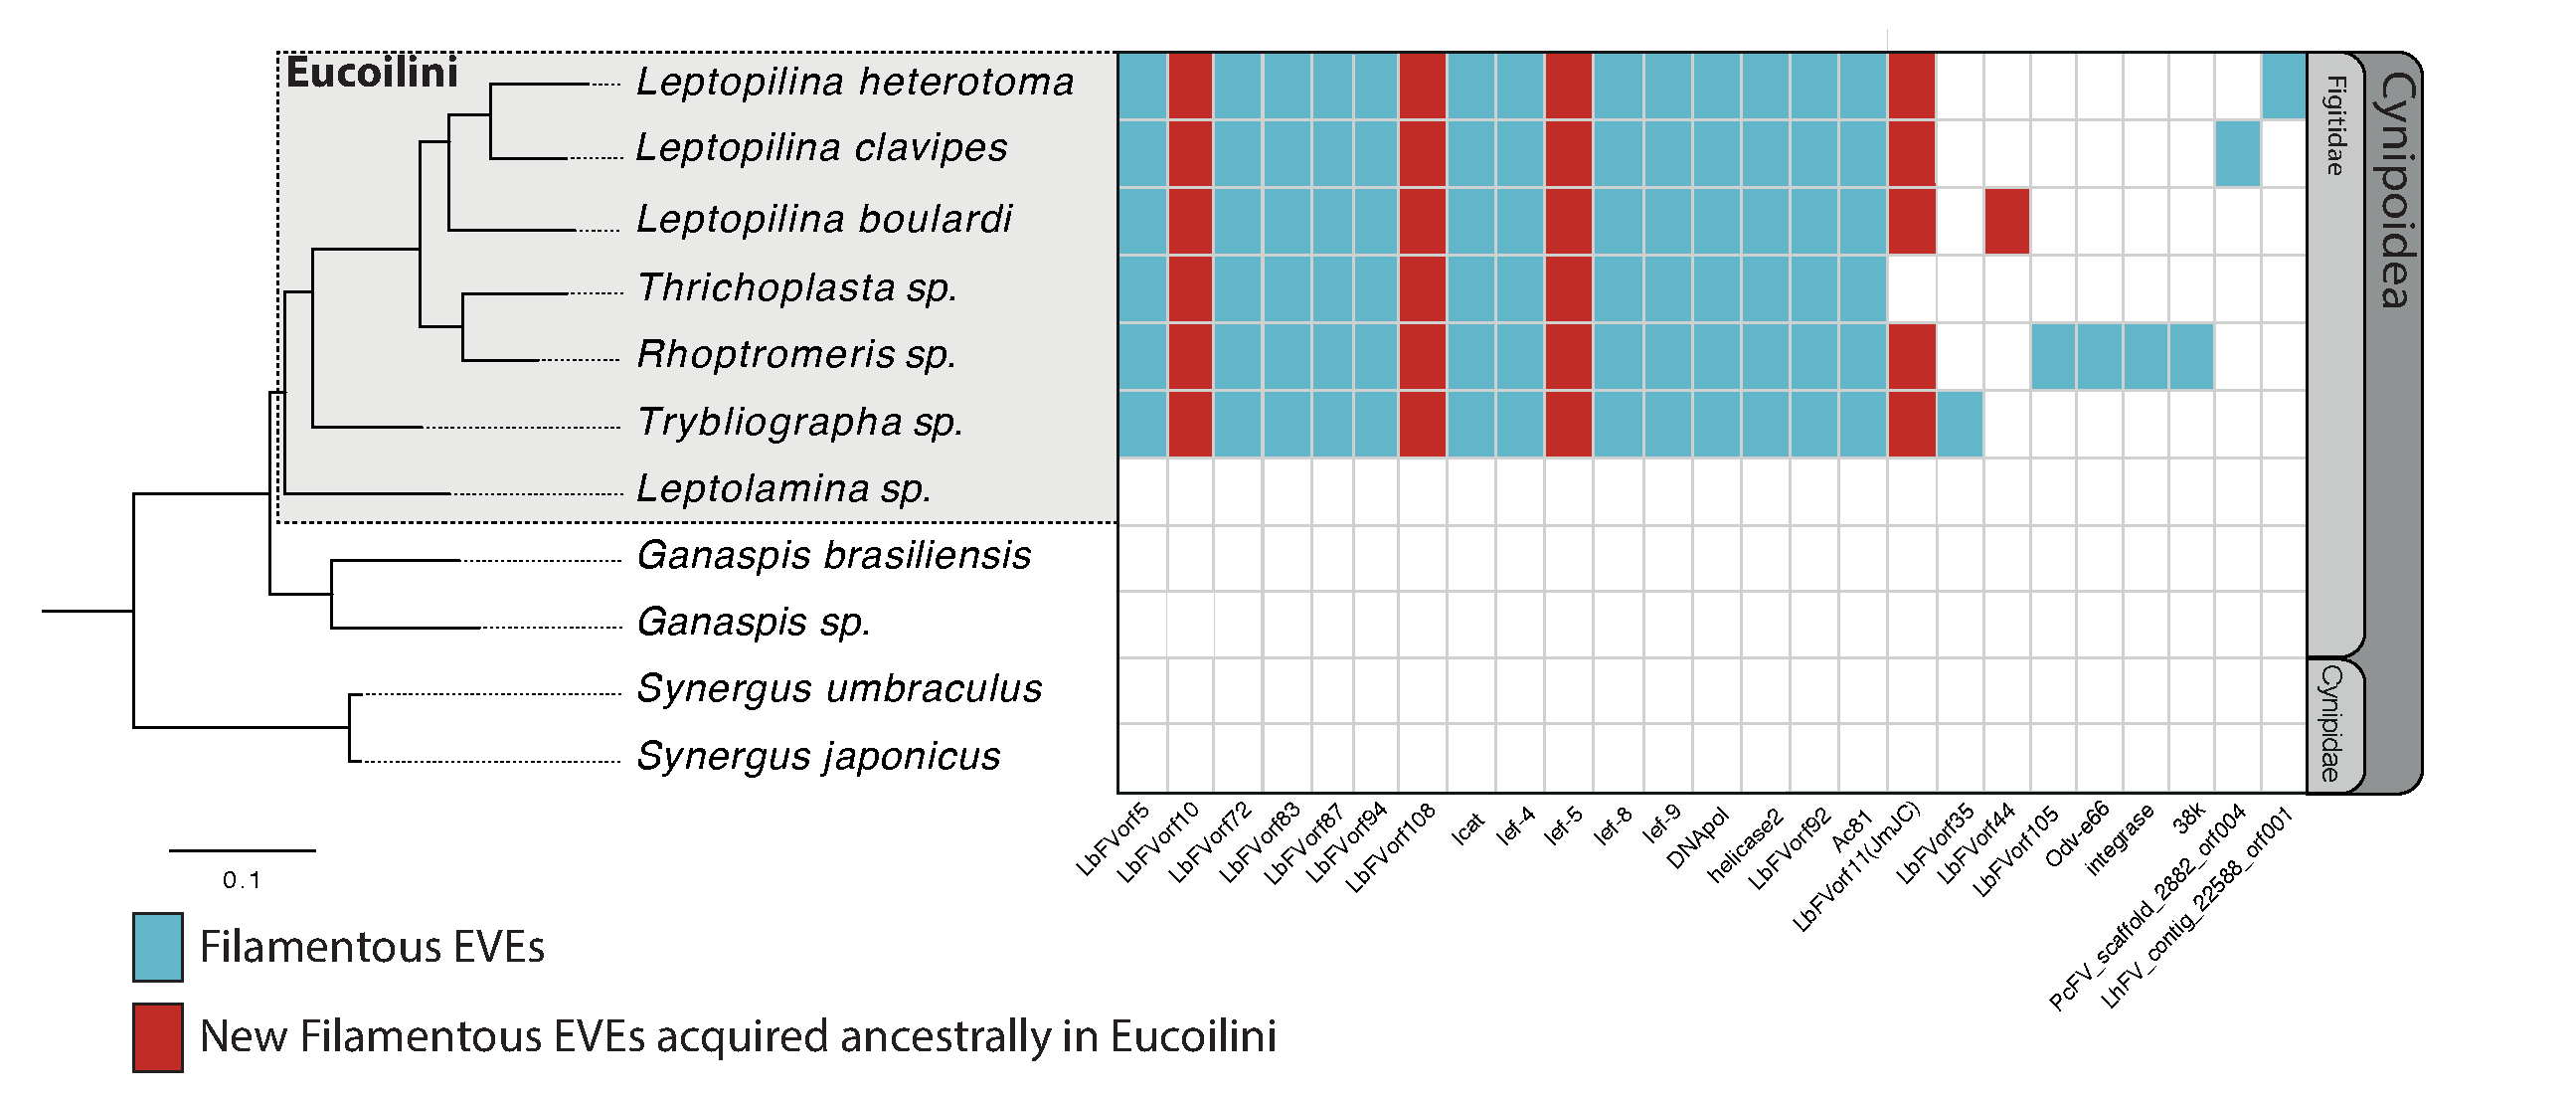
\includegraphics[width=\linewidth,height=\textheight,keepaspectratio]{PhD-master/figures/Cynipoidea_EVE_heatmap.pdf}\centering
\caption[Paper3:Filamentous EVEs distribution in Cynipoideai]{\textbf{Filamentous EVE distribution among Cynipoidea species}.The phylogeny of the Cynipoidea has been estimated using 1,000 Busco genes.
Each blue row represents a Cynipoidea species, whereas each column represents a filamentous EVE.
Blue boxes indicate the presence of EVE in a genome, whereas white boxes indicate its absence. The red boxes indicate the newly assigned EVEs from the same ancestral event as in \cite{di_giovanni_behavior-manipulating_2020}}
\label{figure:Cynipoidea_EVE_heatmap}
\end{figure}


%\subsubsection{\textbf{Filamentous loci are endogenized within Eucoilini genomes}}

In order to check that the 153 putative EVEs were indeed within the genomes of the wasps, i.e. endogenized, we looked at the sequencing coverage profile between scaffolds that contain candidate EVEs and scaffolds containing BUSCO genes (highly conserved genes at the arthropod scale). All scaffolds containing candidate EVEs (n=107 scaffolds) had similar coverage profiles compared to the BUSCO scaffolds  (\figurename{\ref{figure:ALL_cunipids_species_Cov_GC}}), confirming their endogenization. Another way to test the integrated nature of candidate EVEs was to look at the genomic environment of EVEs (see MandM for more details). Out of 107 scaffolds containing EVEs, we found 55 scaffolds that effectively revealed the presence of at least one typical eukaryotic gene or transposable element in the vicinity of the EVEs, further suggesting that they are part of the chromosomes of the wasps. 
%, these results strongly suggest that the filamentous-like genes are part of the wasp genomes. 

\begin{figure}[!htpbt]
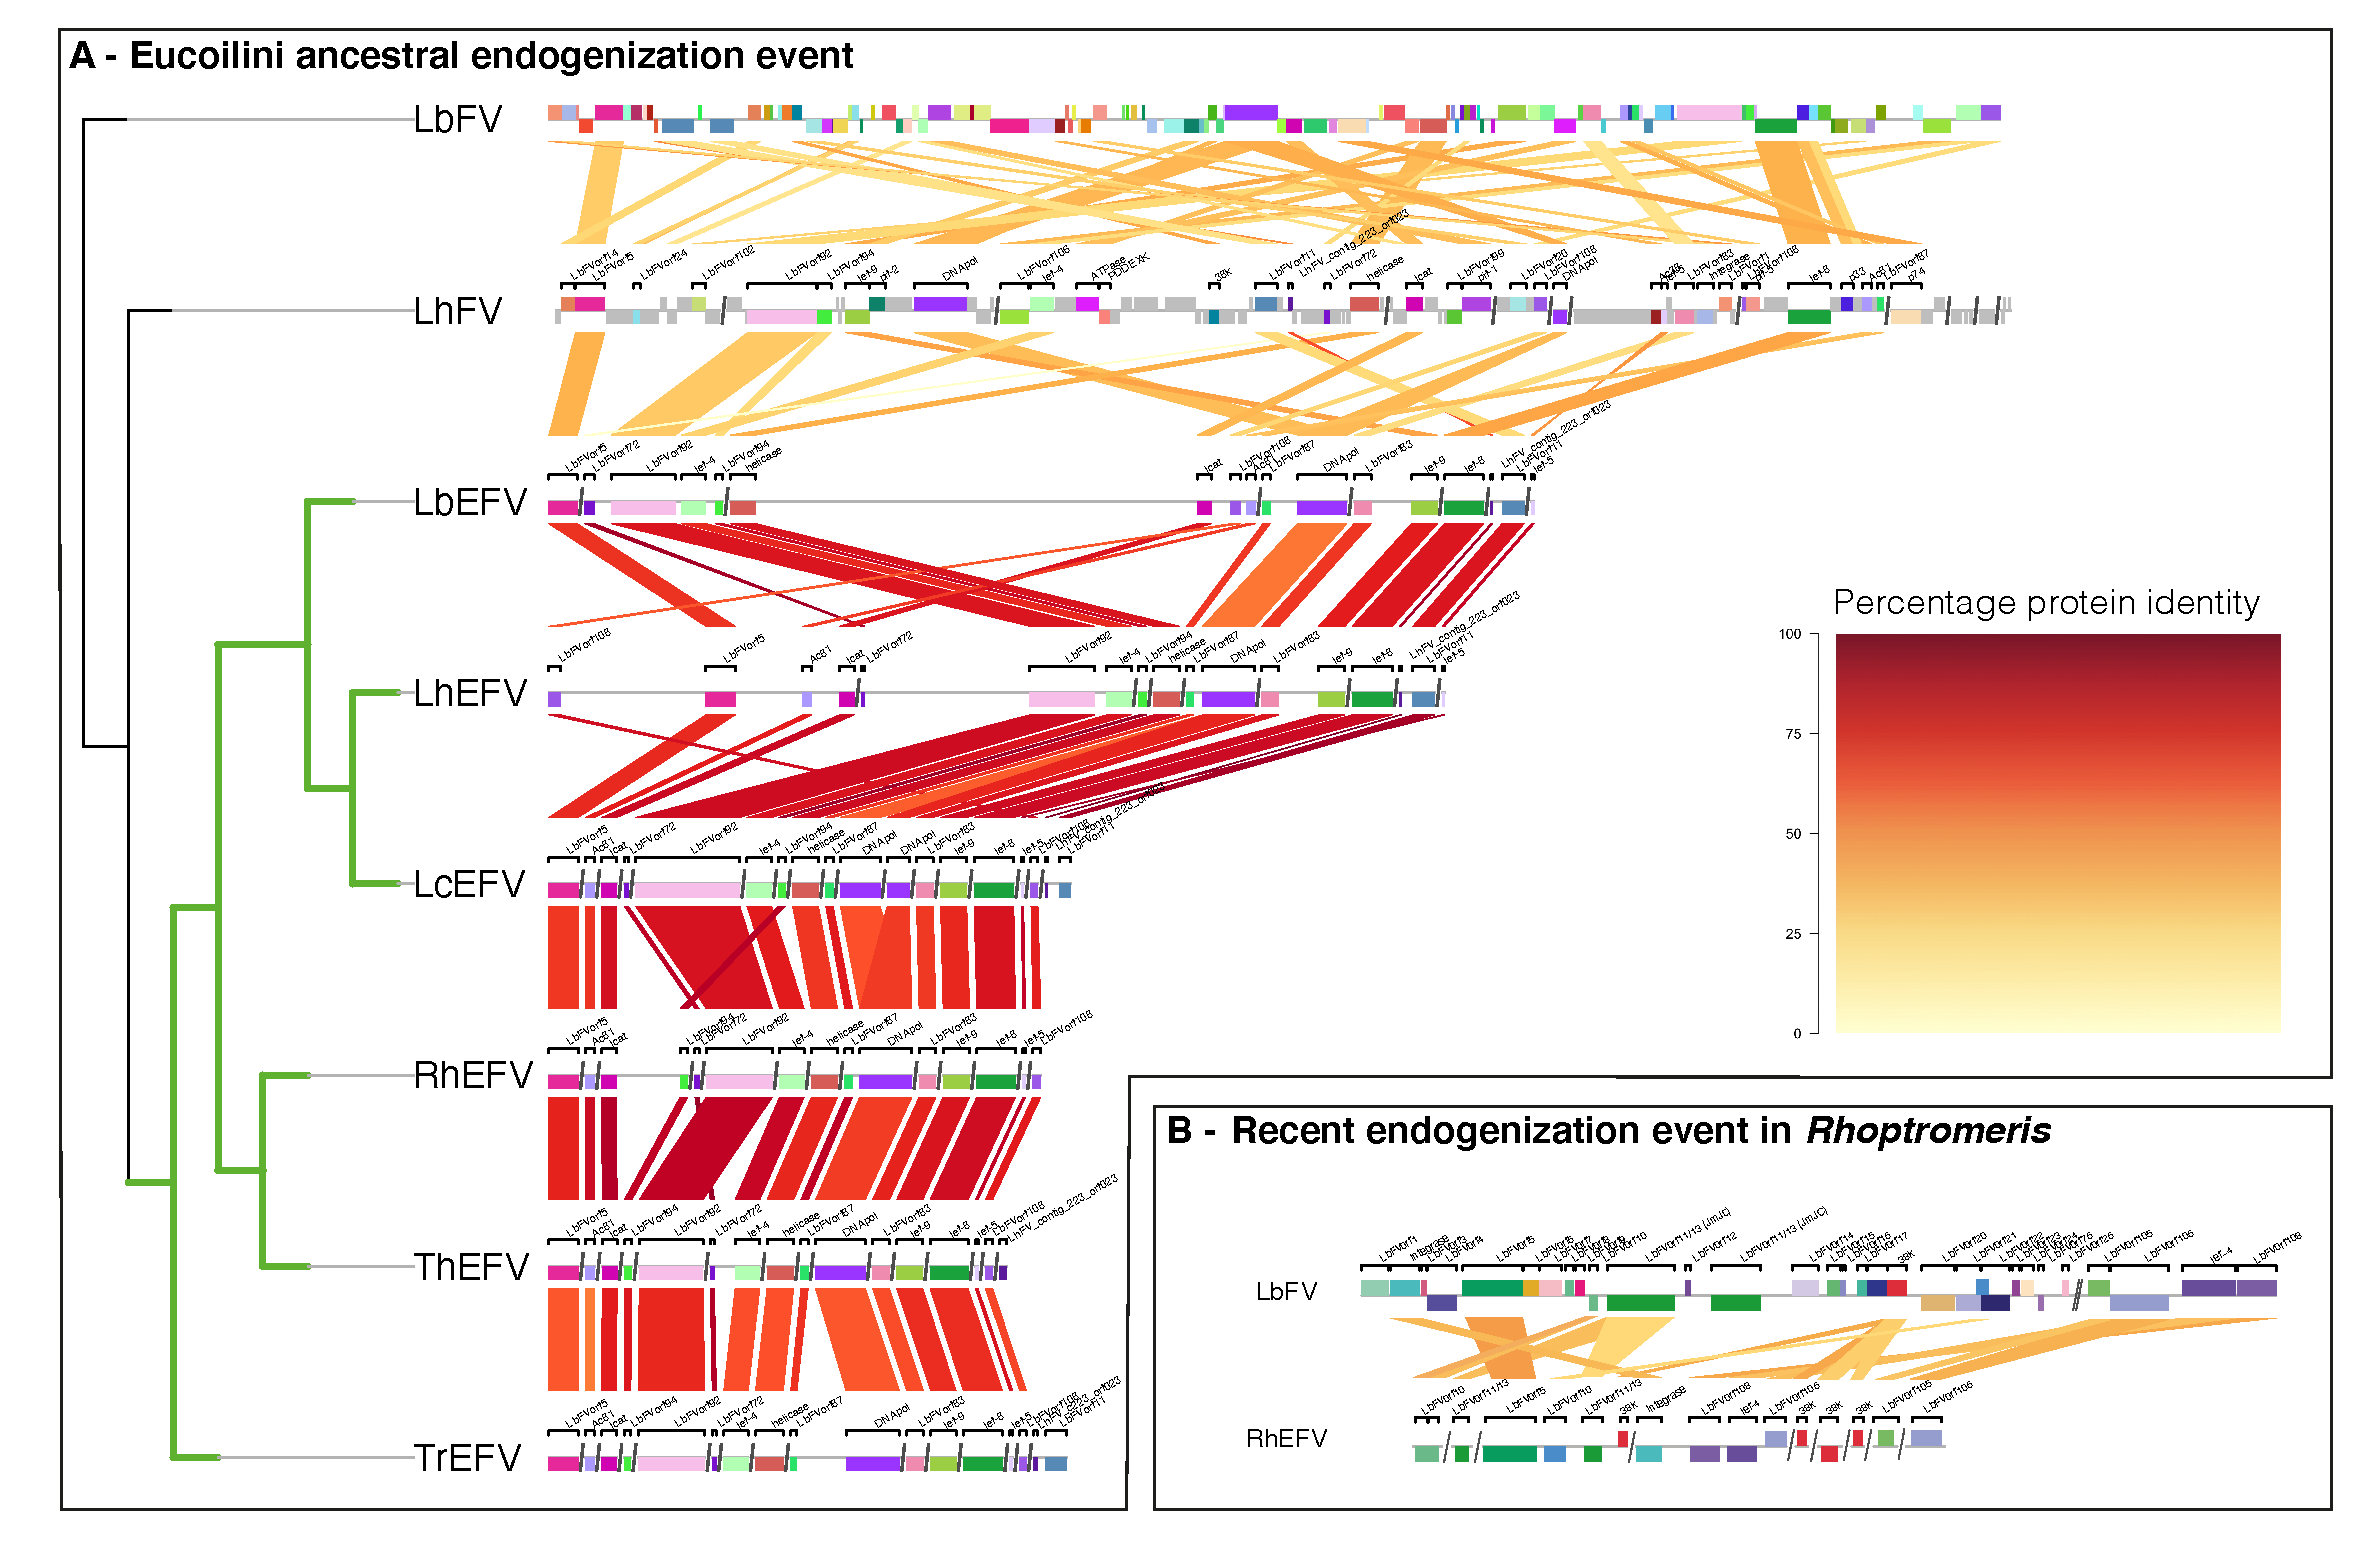
\includegraphics[width=\linewidth,height=\textheight,keepaspectratio]{PhD-master/figures/comparative_genomics_phylo2.pdf}\centering
\caption[Paper3:Filamentous EVE synteny in Eucoilini]{\textbf{Comparative genomics of wasp scaffolds sharing similarities with filamentous ORFs}. Lb, \textit{Leptopilina boulardi}; Lh, \textit{Leptopilina heterotoma}; Lc, \textit{Leptopilina clavipes}. The species tree on the left has been obtained using a concatenation of 541 universal arthropod genes. Green and black branches correspond to Eucoilini and Filamentous branches, respectively. The red/yellow color code depicts the percentage of protein identity between homologous sequence pairs (viral or virally derived loci). Blue boxes identify the virally derived genes and their orientation (above: sense, below: antisense), whereas genes of eukaryotic origin are depicted in gray on the scaffolds. Gray connections indicate homology between nonvirally derived regions. The figure has been drawn using the genoPlotR package \citep{guy_genoplotr_2010}. The scaffolds are ordered from left to right in an arbitrary manner.}
\label{figure:comparative_genomics_Cynipoidea_phylo}
\end{figure}


\begin{landscape}

\begin{figure}[!htpbt]
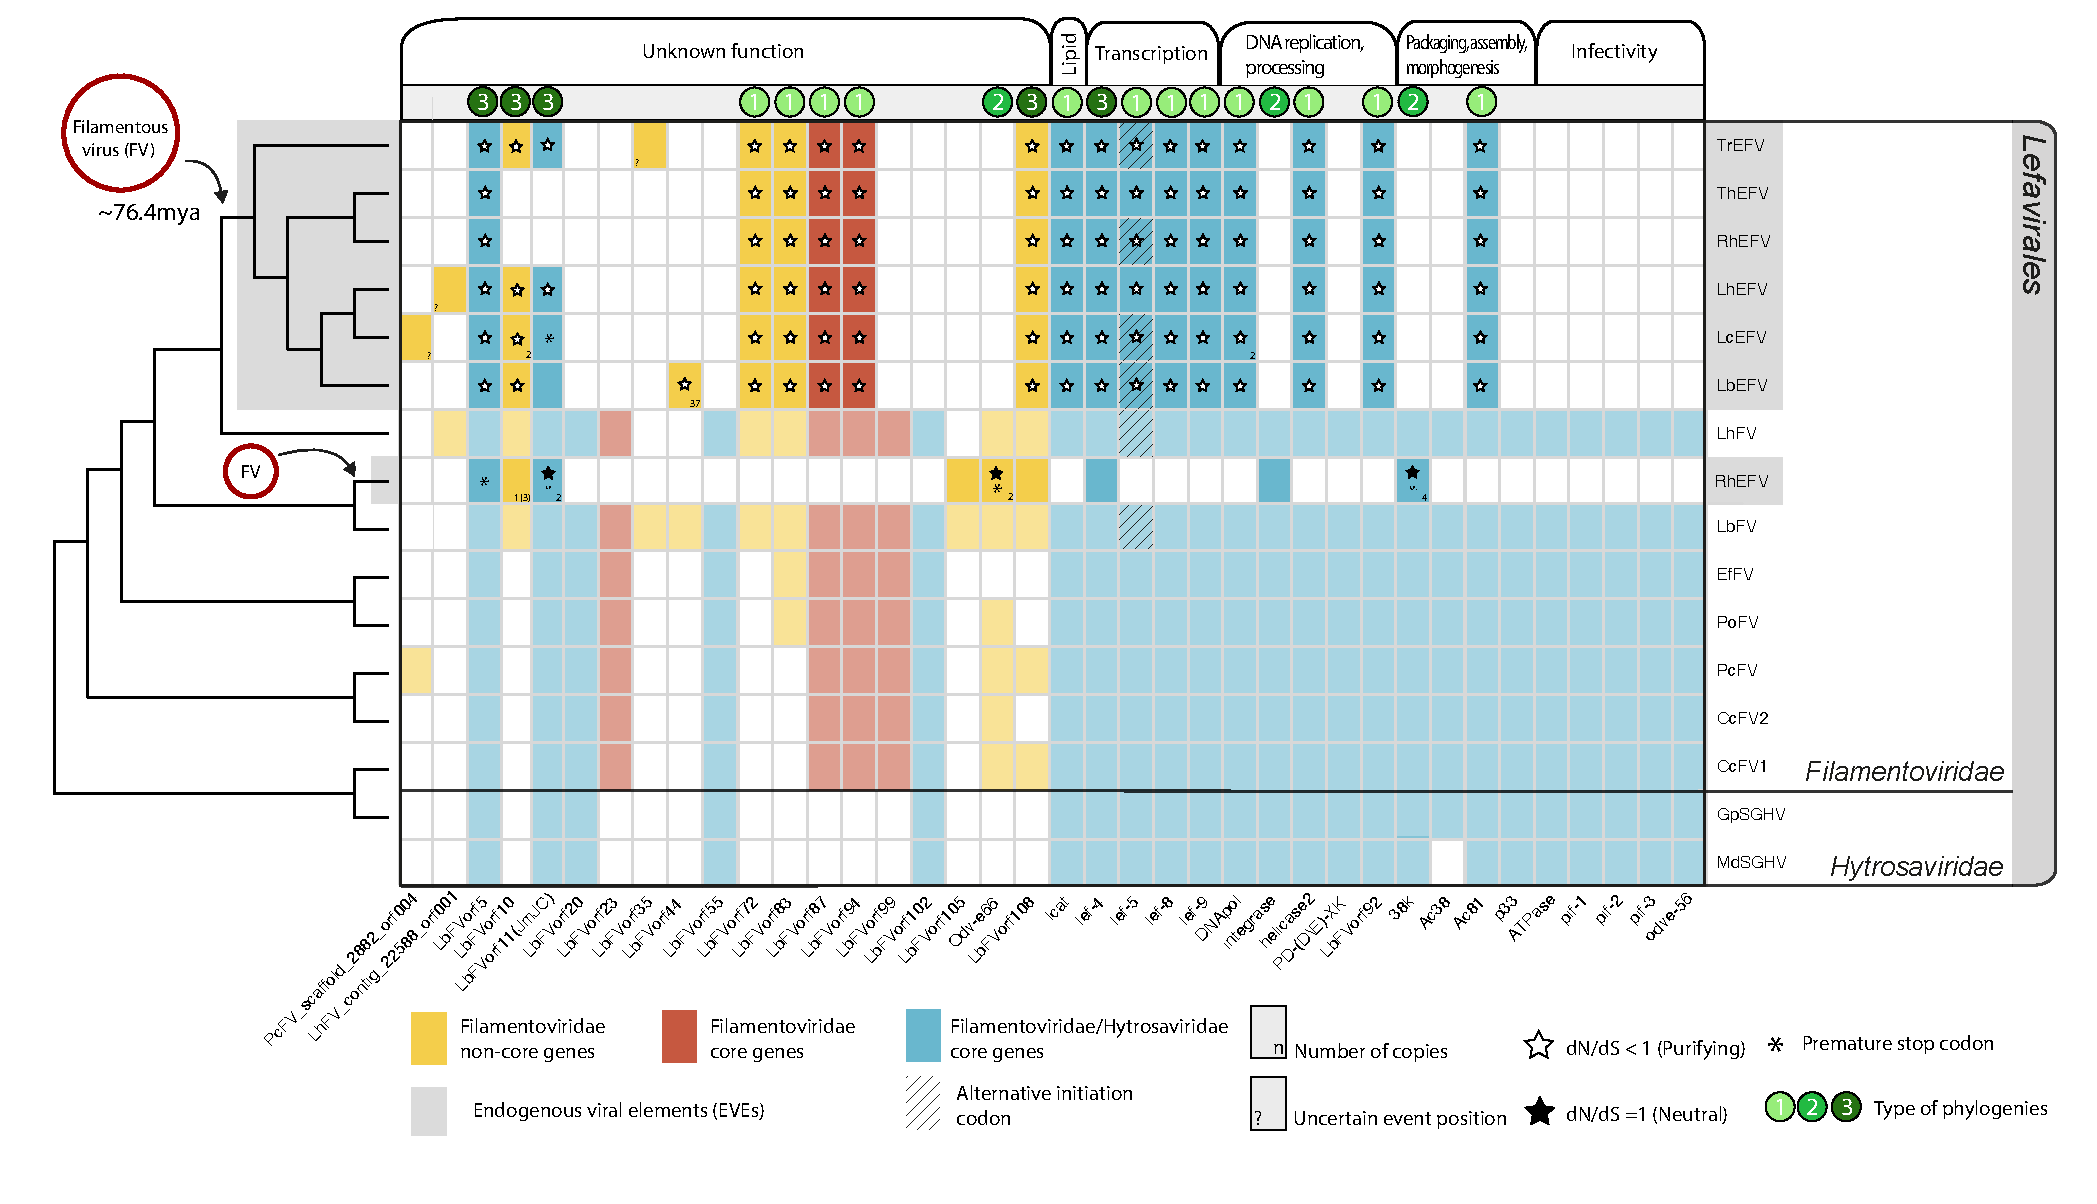
\includegraphics[width=\linewidth,height=\textheight,keepaspectratio]{Heatmap_gene_content.pdf}\centering
\caption[Paper3:Filamentous EVEs distribution in Eucoilini]{\footnotesize\textbf{Gene content heatmap among \textit{Hytrosaviridae} and filamentous genomes as well as endogenous filamentous elements within Eucoilini genomes}. A cladogram phylogeny is reported on the right. The rows represent the viral species, and the columns represent the genes distributed according to their potential functions. A colored box indicates the presence of a gene. Blue represents core genes of filamentous and hytrosavirus, red represents a  core gene in filamentous, and yellow represents non-core genes. When the box is hashed, it indicates that the predicted ORF has an alternative start codon. A star represents EVEs subjected to purifying selection pressure (\textit{dN/dS}$<$1). An asterisk correspond to the presence of premature stop codons in the EVEs. When an asterisk is split in two, it means that part of the EVEs have stop codons, while the other part has complete ORFs. When multiple paralog EVEs can be found in a species,  its number is displayed in the bottom left corner. When an EVE could not be assigned to a particular event, a question mark is displayed in the bottom right corner. The green circles with the numbers correspond to the type of the gene topologie among three topologies types displayed in \figurename{\ref{figure:Type_EVE_phylogenies}}.}
\label{figure:Heatmap_gene_content}
\end{figure}

\end{landscape}

\begin{figure}[!htpbt]
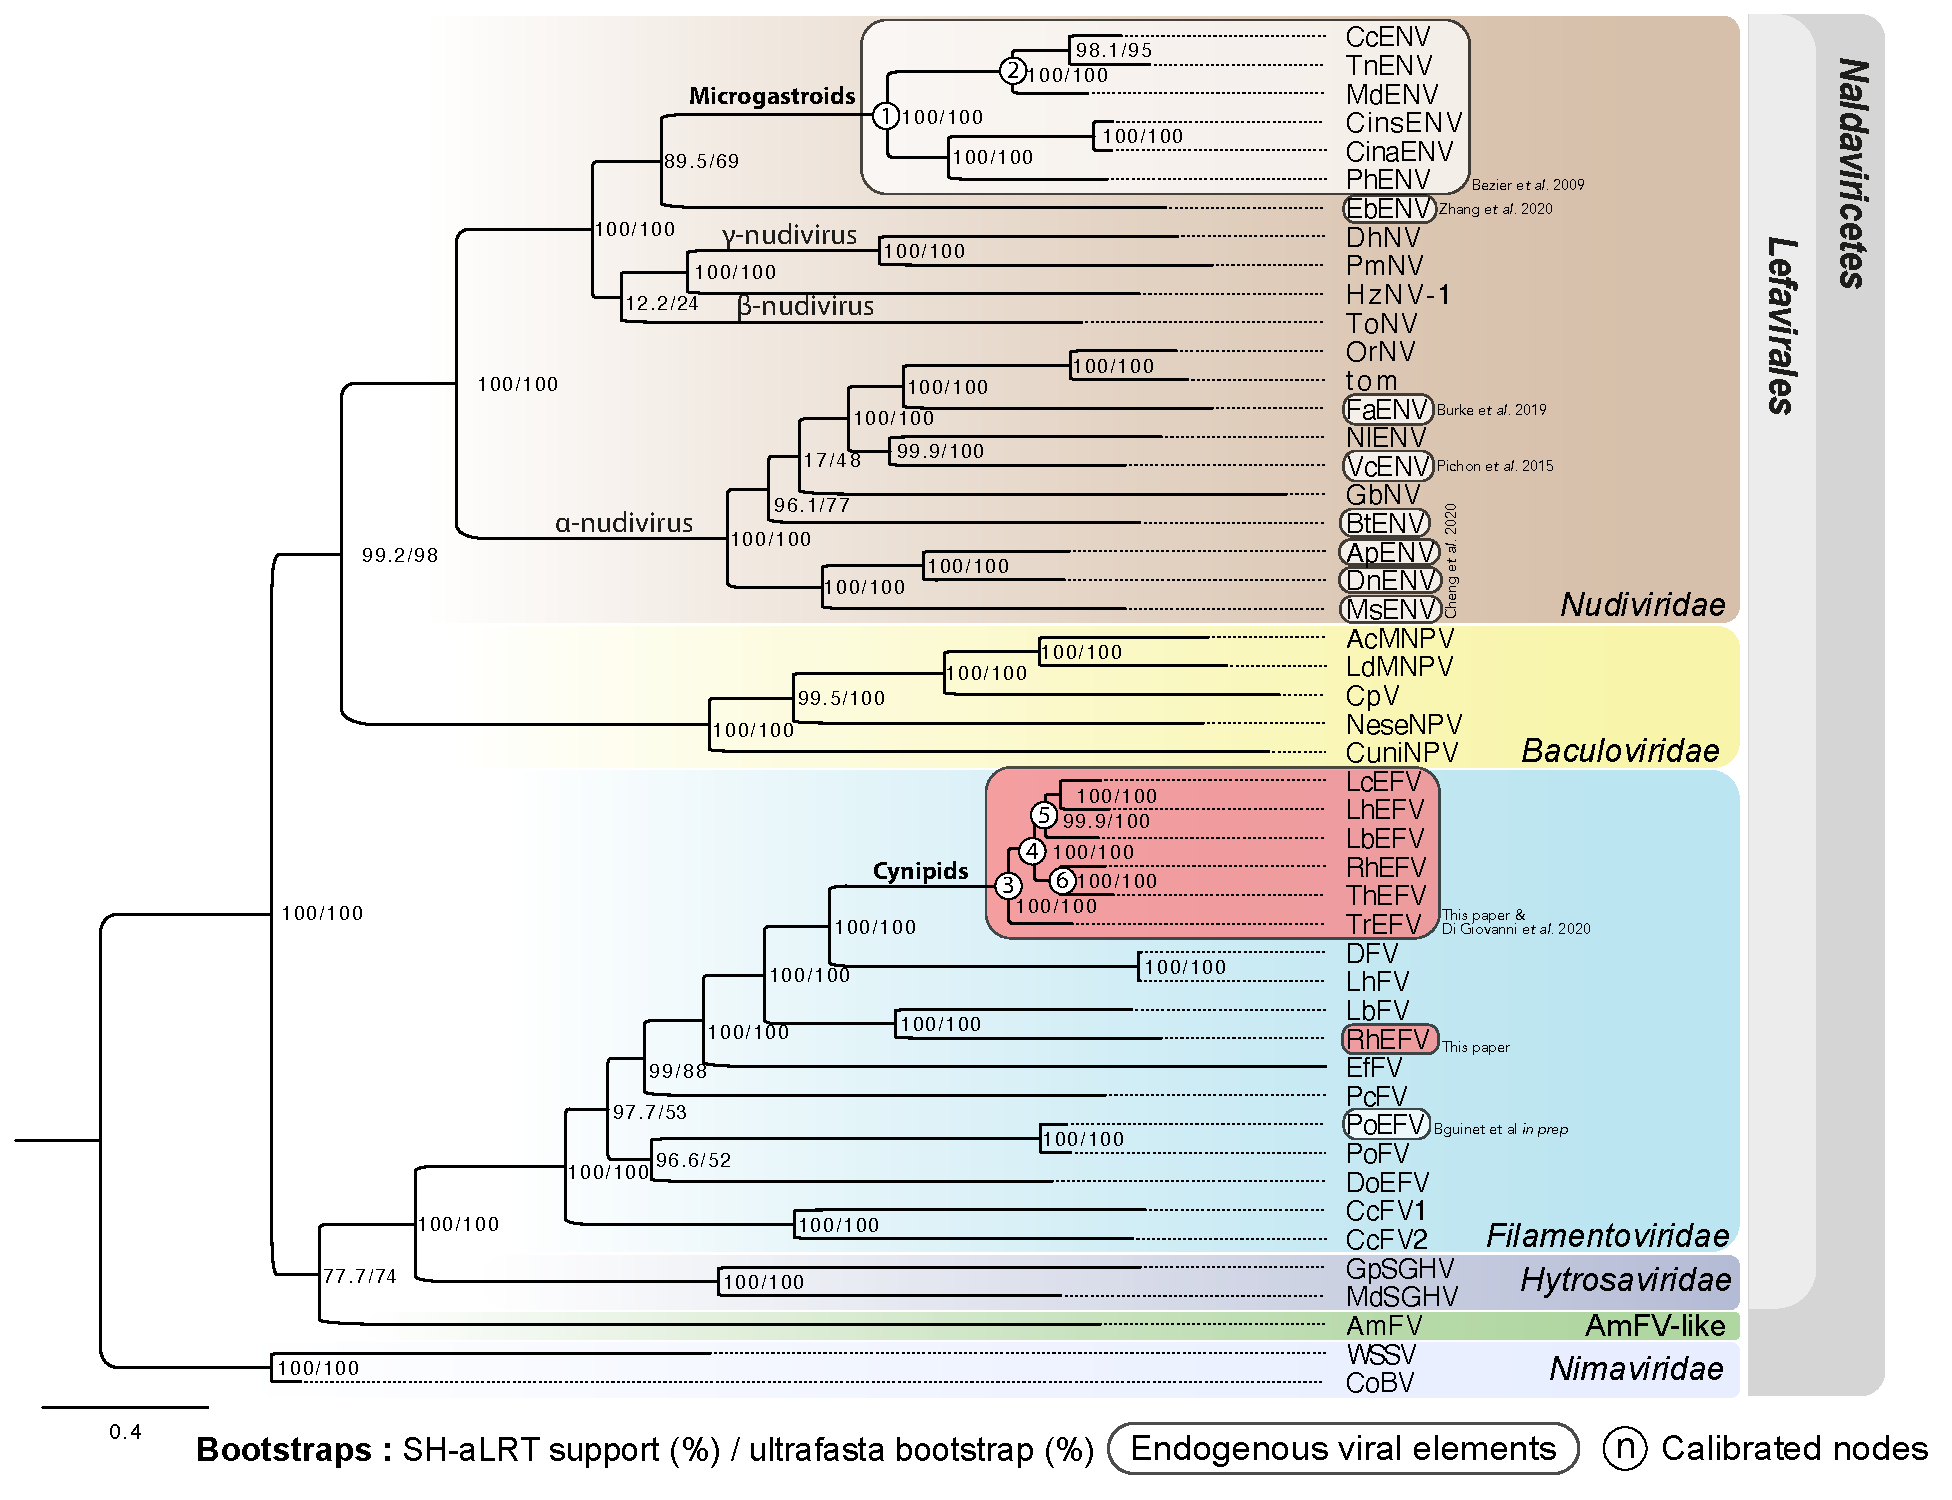
\includegraphics[width=\linewidth,height=\textheight,keepaspectratio]{dsDNA_phylogeny_cynipoidea.pdf}\centering
\caption[Paper3:\textit{Naldaviricetes} phylogenenetic tree including Eucoilini]{\textbf{Phylogenetic tree inference of the \textit{Naldaviricetes}}. The phylogeny wasinferred by maximum likelihood with 113 concatenated amino-acide sequences (25,382 amino-acides sites including only homologous clusters with at least 4 sequences) of 47 viruses. Viruses includes free-living viruses from the families \textit{Baculoviridae}, \textit{Nudiviridae}, \textit{Hytrosaviridae}, \textit{Nimaviridae}, Filamentoviridae and the AmFV virus. 
All previously documented viral endogenization events are highlighted in white boxes, while the newly described events in this paper are highlighted in red boxes.}
\label{figure:dsDNA_phylogeny_cynipoidea}
\end{figure}

\subsection{Two independent integration of filamentous virus occurred in Eucoilini.}

Overall, we could characterize the presence of 25 endogenous filamentous viral genes within the 6 Eucoilini genomes (for a total of 153 EVEs spread across species). To gain insights into their individual history, we constructed phylogenies for each of them. Three types of topologies were observed (\figurename{\ref{figure:Type_EVE_phylogenies}}, see suppl mat for the other phylogenies). 

In type1 phylogenies, all Eucoilini sequences form a monophyletic clade reflecting the expected relationship among wasp species but nested within a filamentous virus clade. In these phylogenies, the closest viral relative is LhFV. These phylogenies are consistant with a single endogenization event that occurred before the divergence of the 5 species and that involved a LhFV-like donor.

In type2 phylogenies, a single sequence corresponding to \textit{Rhoptromeris} was nested within a filamentous virus clade. This sequence was typically branching with LbFV. These phylogenies are consistant with a single endogenization event involving 
only \textit{Rhoptromeris} and a LbFV-like donor.

In type3 phylogenies, we observed both patterns (types 1 \& 2) together. These phylogenies are consistant with an endogenization event that occurred in the common ancestor of the Eucoilini species (as in type 1) and a second event that occurred in the branch leading to \textit{Rhoptromeris} and that involved a LbFV-like donnor (as in type 2). 

Out of the 20 gene phylogenies that could be classified this way, 14 presented the type1, 5 the type2 and 2 the type3. The remaining genes could not be classified this way because they had too few leaves.  All filamentous gene phylogeny figures can be found in the file : \href{https://github.com/BenjaminGuinet/PhD_defense/blob/main/Supplementary_paper3/ALL_Eucoilini_filamentous_phylogenies.pdf}{ALL\_Eucoilini\_filamentous\_phylogenies.pdf}. 
We then used the genomic location of the EVEs to aggregate them into single events. Our rationale was that EVEs that are physically close to each other (i.e. in the same contig) are likely to have been acquired together during the same endogenization event (connected EVEs = 71/153). Using both the phylogenetic and physical informations combined, we were able to aggregate 152/153 EVEs into 2 events. Within each event, the gene phylogenies were congruent, as expected if they do have the same evolutionary history. \\


\begin{figure}[!htpbt]
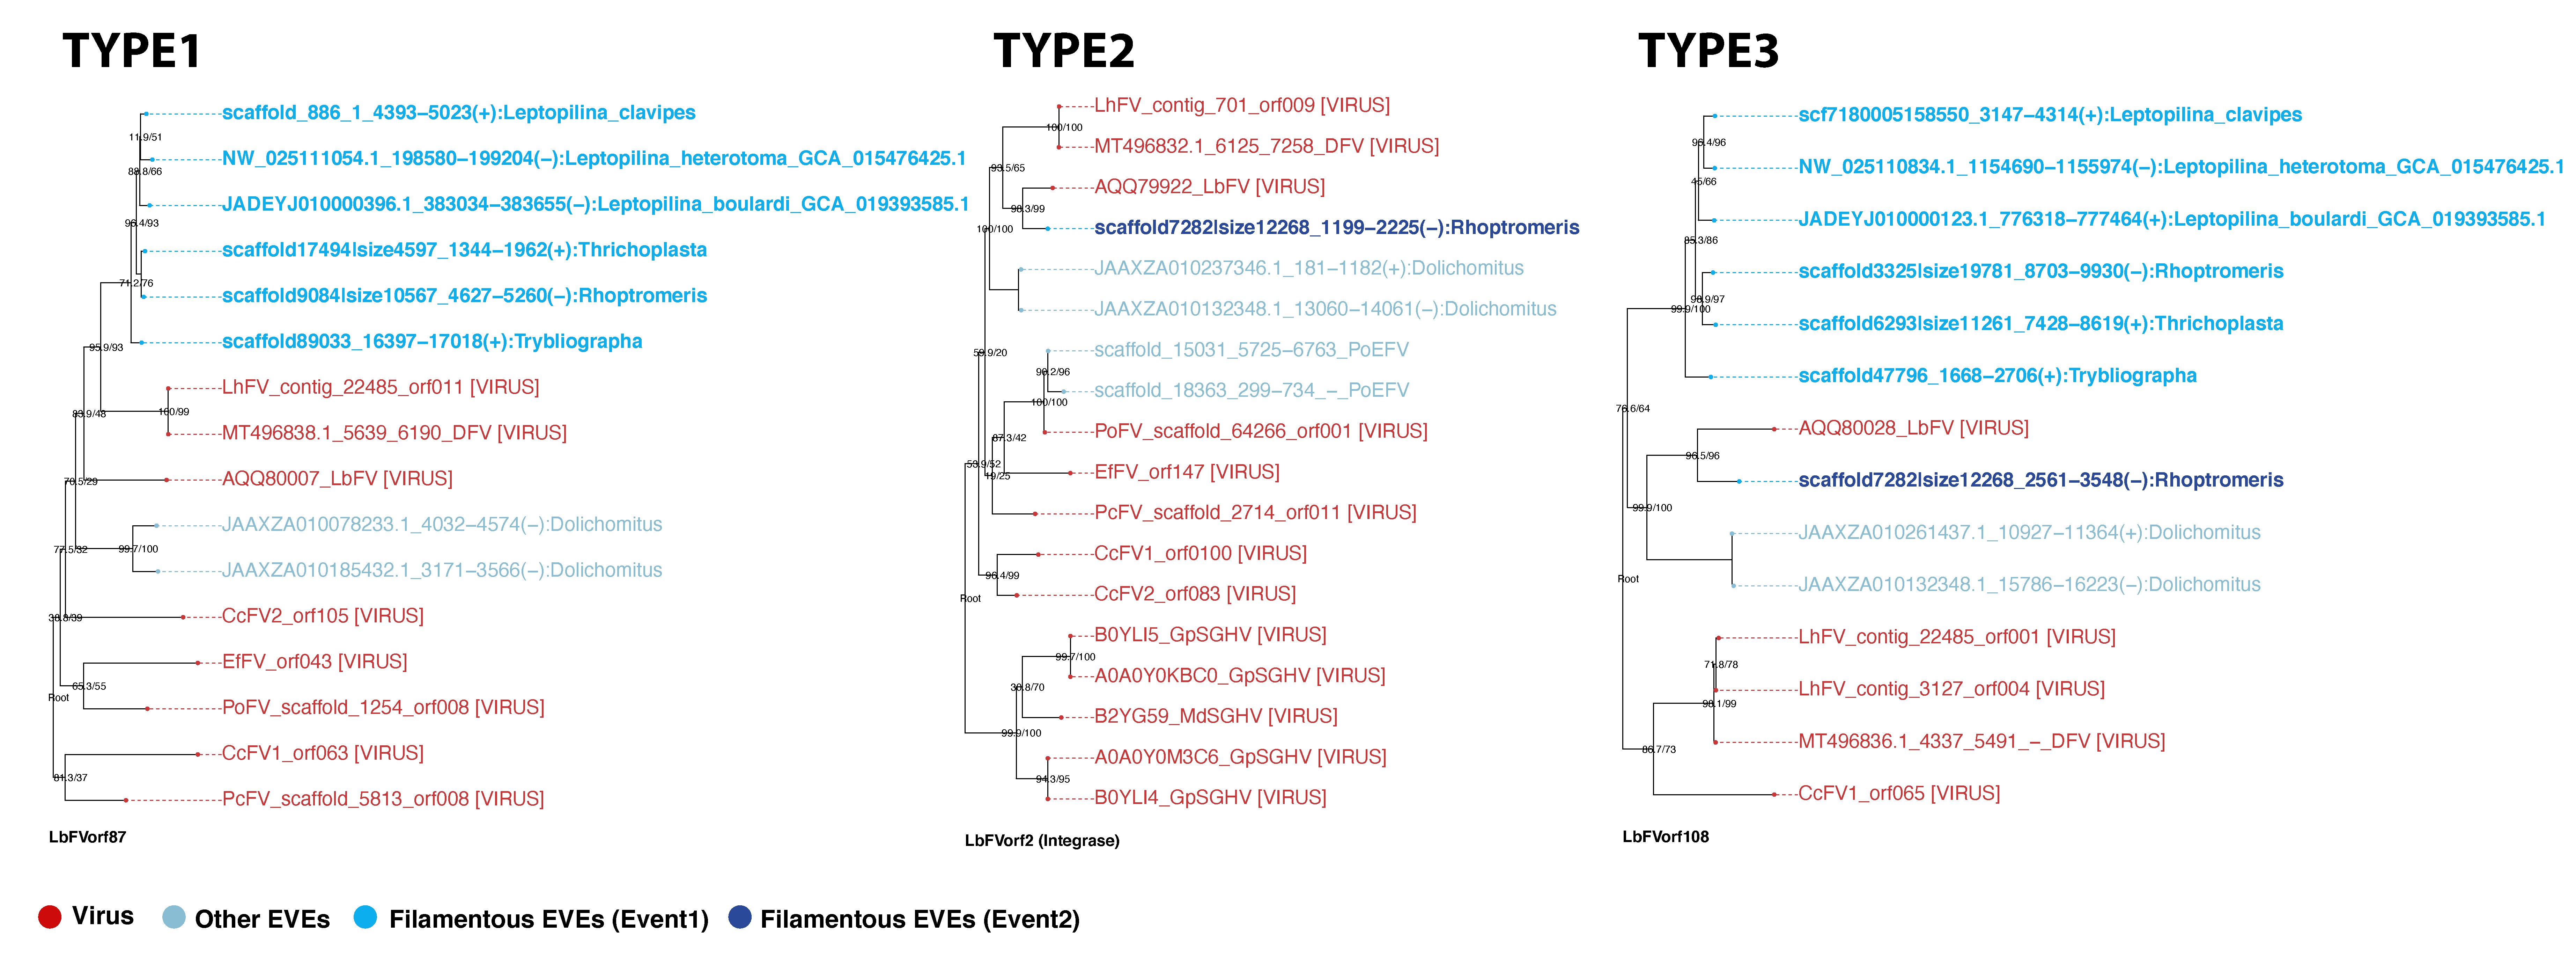
\includegraphics[width=\linewidth,height=\textheight,keepaspectratio]{PhD-master/figures/Type_EVE_phylogenies.pdf}\centering
\caption[Paper3:Type of Eucoilini EVE phylogenies]{\textbf{Example of phylogenies observed}. The type1 corresponds to a single endogenization event that occurred in the ancestor of all Eucoilini species and involving a LhFV-like donor. The Type2 suggest another independant event that occurred in the \textit{Rhoptromeris} branch involving a LbFV-like donor. The type3 phylogenies suggest that both events occurred.}.
\label{figure:Type_EVE_phylogenies}
\end{figure}


\textbf{First endogenization event within the Eucoilini common ancestor}

The first event was the most ancient, as it involves an endogenization that occurred in the common ancestor of the 6 Eucoilini species. We were able to aggregate 18 filamentous genes in this event, including the 13 genes already identified as domesticated in \textit{Leptopilina} species (Di Giovanni et al., 2020). Among the 18 filamentous genes, 17 were present in all Eucoilini species, and formed a clear monophyletic clade nested within filamentous viruses (see supplementary phylogeny). A phylogeny based on the concatenation of these genes produced the same phylogenetic signal, with each Eucoilini species forming a highly supported monophyletic clade (bootstrap=100), with LhFV as the closest filamentous virus (\figurename{\ref{figure:dsDNA_phylogeny_cynipoidea}}).  

Compared to previous study (Di Giovanni et al., 2020), we identified five additional ancestrally acquired genes, three of which were currently shared by all Eucoilini. These genes and their putative functions are presented below (all the gene phylogenies as well as sequence alignments are available in PDF files under the respectively following GitHub files : \href{https://github.com/BenjaminGuinet/PhD_defense/blob/main/Supplementary_paper3/ALL_Eucoilini_filamentous_phylogenies.pdf}{ALL\_Eucoilini\_filamentous\_phylogenies.pdf} and \href{https://github.com/BenjaminGuinet/PhD_defense/tree/main/Supplementary_paper3/All_Eucoilini_filamentous_alignments}{ALL\_Eucoilini\_filamentous\_alignments}.

\textbf{LbFVorf108} is a non-filamentous core gene present only in LbFV, LhFV, CcFV1 and PcFV genomes (\hyperref[sec:chap2]{chapitre 2}:\textit{in prep}) with no known homologs in public databases. This gene was detected in \textit{L.boulardi} and \textit{L.heterotoma} scaffolds containing other filamentous genes, previously identified by (Di Giovanni et al., 2020). This result strongly suggests that they derive from the same endogenization event (\figurename{\ref{figure:comparative_genomics_Cynipoidea_phylo}}-A). Since all Eucoilini EVEs had a complete open reading frame and were under strong purifying selection, LbFVorf108 is very likely functional in Eucoilini genomes (mean \textit{dN/dS}=0.2792 (SE=0.03)). The gene phylogeny further suggests a second event of endogenization in \textit{Rhoptromeris} (see below).\\

\textbf{LbFVorf10} EVE was found endogenized in all Eucoilini species except \textit{Thrichoplasta}. 3 LbFVorf10 paralog EVEs were found in 2 \textit{Rhoptromeris} scaffolds (scaffold10766 and scaffold32196) in which other EVEs were present in the case of scaffold10766 (LbFVorf5, LbFVorf11/13 and 38k). However, we cannot conclusively establish that the two EVEs in scaffold32196 are integrated because the mean coverage depth of this scaffold differs significantly from the distribution of the BUSCO coverage depth scaffolds (BUSCO=51.7X, scaffold32196=22X, pvalue= 0.0007). These two EVEs could then possibly correspond to EVEs from a free-living filamentous virus, although this is unlikely given that we do not find any other scaffold with such exogenous evidence. These 2 scaffolds contained EVEs clearly part of an independent endogenization event from the initial event involving multiple Eucoilini species (described in detail below). This result suggests that LbFVorf10  was probably integrated into the common ancestor of Eucoilini, and was then lost in the \textit{Rhoptromeris} genome, while another copy was brought from a second event and probably undergone two duplication events (more details on this second event are given in the next section). A micro syntenic block involving \textbf{LbFVorf10} and LbFVorf11 was observed among  all four species involved in the first event (\figurename{\ref{figure:comparative_genomics_Cynipoidea_phylo}}-A), further supporting the common origin of these loci. Surprisingly, the same association was found in the second event (\figurename{\ref{figure:comparative_genomics_Cynipoidea_phylo}}-B).
Interestingly, a HHpred analysis on the amino-acide alignment against the PDB\_mmCIF70\_12 db predicted a homology with a Glycoprotein containing a Zinc finger domain from a Hantavirus protein (Evalue 5.9e-8) (\figurename{\ref{table:ORF_functions}}). Besides, all LbFVorf10 EVEs presented a complete ORF. A \textit{dN/dS} analysis on the EVEs from the ancestral Eucoilini event clearly showed strong purifying selection (mean \textit{dN/dS}=0.1654 (SE=0.033), while the \textit{dN/dS} on the 3 \textit{Rhoptromeris} paralogs did not succeed to reject the null hypothesis of a neutral regime (mean \textit{dN/dS}=0.442 (SE=0.34, pvalue=0.143).\\


\textit{\textbf{Lef-5}} EVE was not previously predicted in the LbFV genome due to its alternative start codon TTG also present in the LhFV \textit{lef-5} gene (\hyperref[sec:chap2]{chapitre 2}:\textit{in prep}). Interestingly, alternative start codon TTG can also be found in the \textit{lef-5} EVEs in \textit{Rhoptromeris}, \textit{Leptopilina boulardi} and \textit{Trybliographa} genomes. Predicting ORF with this start alternative codon, we clearly found the same conserved domain in the upstream region as with the other sequences with an ATG start codon. Furthermore, we did not find any open reading frames involving an ATG codon in the \textit{L.boulardi} genome. These results therefore suggest that these alternative codons do have biological significance. We also find an alternative start codon CTG for \textit{Leptopilina clavipes} which also includes the upstream conserved domain. On the other hand, \textit{Leptopilina heterotoma} and \textit{Thrichoplasta} genomes had a classic ATG start codon. Overall, these results indicate a complex evolution of the initiation codon in Filamentoviridae and in EVEs found in Eucoilini wasps. Nevertheless, additional analysis using transcriptomic data are needed to shed light on this question. Lastly, in all Eucoilini genomes, the \textit{lef-5} was always found isolated in scaffolds, without any other EVEs. All EVEs were composed of complete open reading frames and showed strong purifying selection at these loci (mean \textit{dN/dS}=0.1118 (SE=0.03)). The filamentous \textit{lef-5} EVE might be involved in RNA polymerase initiation  transcription factor as in baculoviruses \citep{su_autographa_2011}\\ 

\textbf{LbFVorf11 (JmJC)} was detected in all the Eucoilini species except \textit{Thrichoplasta}. 3/5 gènes present incomplete ORFs or premature stop codon.  The phylogeny of this gene supported two independent integration events. One in \textit{Rhoptromeris} followed by a probable duplication (bootstrap = 100, see supplementary phylogeny fig-\href{https://github.com/BenjaminGuinet/PhD_defense/blob/main/Supplementary_paper3/ALL_Eucoilini_filamentous_phylogenies.pdf}{S1}). A \textit{dN/dS} analysis shows that these sequences evolve under a neutral regime. Additionnally, one independent event occurred in the common ancestor of \textit{L.clavipes}, \textit{L.heterotoma}, \textit{L. boulardi} and \textit{Trybliographa} (boostrap = 100, see supplementary phylogeny fig-\href{https://github.com/BenjaminGuinet/PhD_defense/blob/main/Supplementary_paper3/ALL_Eucoilini_filamentous_phylogenies.pdf}{S1}). For these endogenized genes, the \textit{dN/dS} analysis suggests a purifying regime of selection (mean \textit{dN/dS}=0.1325, (SE= 0.016)), suggesting that at least the copies with complete ORF in \textit{L.heterotoma} and \textit{Trybliographa} could still be functional. In addition, these genes likely arrived at the same time as the other genes, since this gene is present in scaffolds containing other filamentous genes in all 4 Eucoilini genomes. (\figurename{\ref{figure:comparative_genomics_Cynipoidea_phylo}}-A). Intriguingly, the phylogeny suggests that the filamentous \textit{JmJC} gene itselfs has a eukaryotic origin. Indeed, the phylogeny is composed of numerous eukaryotes that form an almost monophyletic clade (with a single exception out of x branches, which may in fact correspond to an EVE in another Hymenoptera), within which a well supported clade containing the Filamentoviridae and the wasps is nested. This suggests a two-step integration event from eukaryotes to filamentous viruses and then to the wasp's genomes (see supplemental phylogeny).\\

\textbf{LbFVorf44} EVE was only found within the \textit{Leptopilina boulardi} genome. Still, the gene seemed to belong to the first event. Indeed, this gene contained 37 paralog EVEs distributed within 23 \textit{L.boulardi} scaffolds (see supplementary phylogeny fig-\href{https://github.com/BenjaminGuinet/PhD_defense/blob/main/Supplementary_paper3/ALL_Eucoilini_filamentous_phylogenies.pdf}{S13}). Among them, one was present in the same scaffolds as the LbFVorf96 (\textit{lef-8}), which is part of the first endogenization event. This suggests that the original copy of this locus was located in this genomic region  (scaffold JADEYJ010000341) and was then duplicated. Among the 37 EVEs, 29 presented a complete open reading frame and a \textit{dN/dS} analysis showed a purifying selection among the paralogs (mean \textit{dN/dS}=0.3004, (SE= 0.077)). This gene has no known homologs in public databases.\\

\textbf{Second endogenization event unique to the \textit{Rhoptromeris} genome}

Concerning the second event, which only concerned the \textit{Rhoptromeris} species, we managed to associate 9 filamentous genes (n=14 EVEs) (\figurename{\ref{figure:comparative_genomics_Cynipoidea_phylo}}-B), 3 of which (LbFVorf5, LbFVorf108 and \textit{lef-4}) were present in two copies (one copy brought by the first event and another by the second event). 4/9 of these genes were only found in \textit{Rhoptromeris} (LbFVorf105, LbFVorf106, \textit{Integrase} and 38k)(\figurename{\ref{figure:Heatmap_gene_content}}). The phylogeny based on the concatenation of these genes placed \textit{Rhoptromeris} outside the Eucoilin clade, right adjacent to the LbFV species, supporting the hypothesis that these genes were acquired from another independent event involving a virus related to LbFV (\figurename{\ref{figure:dsDNA_phylogeny_cynipoidea}}). \\

Among the EVEs, 7 out of 14 contained a premature stop codons or open reading frames and were considered too small to be functional (\figurename{\ref{figure:Heatmap_gene_content}}).

Interestingly, the 7 other EVEs (LbFvorf108, LbFVorf11/13 (\textit{JmJC}), LbFVorf106 (\textit{odv-e66}), LbFV\_contig223\_orf23, \textit{lef-4}, \textit{38k}, and \textit{Integrase}) presented complete open reading frames, meaning that they could still be functional in the \textit{Rhoptromeris} genome. The fact that 7 other EVEs had premature stop codons or incomplete ORFs, however, indicates that the moment of integration was sufficiently old to allow nonfunctional EVEs to evolve under a neutral regime and accumulate premature stop codons. Therefore, the lack of a stop codon in the seven genes makes it conceivable that they have maintained their activity due to purifying selection. \\

As seen above, the LbFVorf10 seemed to have replaced the homologous EVE brought by the first event, since no additional copy could be found within the \textit{Rhoptromeris} genome (\figurename{\ref{figure:comparative_genomics_Cynipoidea_phylo}}-A). 

Additionally, we find evidences for a homolog in LbFV genome that includes an alternative start codon (TTG) (coordinates : 21727-22195). Interestingly, the EVE copy of this gene also presented the same alternative start codon TTG within the \textit{Rhoptromeris} genome (see alignment supplementary file). This further support the idea that the LbFVorf10 EVE brought by the first event has been replaced by a second integration event involving a filamentous virus closely related to LbFV. Whether this copy is still functional is unclear and requires further investigation.\\

Interestingly, the \textit{Integrase} and the LbFVorf106 (\textit{odv-e66}) were both uniquely found in the \textit{Rhoptromeris} genome, while they were absent from the other species (\figurename{\ref{figure:comparative_genomics_Cynipoidea_phylo}}-A). Despite the fact that the LbFVorf106 EVE contained both a copy with an intact open reading frame and with a premature stop codon, a \textit{dN/dS} analysis revealed a regime of selection that was not significantly distinct from a neutral regime. In the case of the \textit{Integrase}, no paralogs were found, rendering a \textit{dN/dS} analysis impossible. 

\subsection{All EVEs brought by the first ancestral endogenization event are domesticated}

Among the EVEs presenting at least two homologs in Eucoilini genomes (n=21), we calculated the \textit{dN/dS} ratios using alignments of the 6 Eucoilini sequences to assess the regime of selection at play since their endogenization. As a reference for genes under stabilizing selection, we also calculated \textit{dN/dS} ratios for 1000 genes shared by at least 90\% of all arthropods \citep{simao_busco_2015}. As expected, the "universal" arthropod gene set had a low \textit{dN/dS} mean value (mean=0.098, sd=0.06)(\figurename{\ref{figure:dNdS_position_plot}}). Among the 21 EVEs, 18 filamentous EVEs from the first ancestral event had \textit{dN/dS} values significantly below 1 (mean=0.18, sd=0.084) and within the range of BUSCO genes (\figurename{\ref{figure:dNdS_position_plot}}), suggesting they were all essential for Eucoilini wasp survival and reproduction. However, they had slightly higher \textit{dN/dS} values than the BUSCO genes (T.test two-sided, df=1015 , p-value = 6.442e-09), which could indicate a slightly lower stabilizing selection intensity or adaptive evolution for some sites and/or genes. A total of 2,354/7,233 codons were subject to purifying selection (see supplementary excel table) : Contrast\_FEL\_table). Further, we wanted to determine if any of the filamentous genes exhibited evidence of diversifying selection, which could indicate interaction with host protein. To do so, we conducted a systematic FEL analysis \citep{kosakovsky_pond_not_2005}. Such analysis estimates synonymous (\textit{dS}) and non-synonymous (\textit{dN}) rates site-wise and employs a likelihood ratio test to determine if \textit{dN$>$dS} at a given site. Using a conservative pvalue of 0.05 (compared to the FEL default threshold of 0.1), we were able to estimate that 23 codons were under diversifying selective pressure. These codons were the most abundant within the LbFVorf68 (\textit{helicase2}) and LbFVorf92 (n=4)(\figurename{\ref{figure:dNdS_position_plot}}).

\subsection{Filamentous genome integrated within Eucoilini during the Cretaceous around 76 mya}

%The common evolutionary history of the 18 genes acquired from the same endogenization event in the common ancestor of the 6 Eucoilini species is consistent with a horizontal transmission from a virus related to LhFV. Such hypotheses are supported by a complete co-phylogeny between filamentous viral genes and the Eucoilini phylogeny (\figurename{\ref{figure:Schizophora_Eucoilini_virus_phylogeny}}). 
On the basis of our observations, the timing of the major domestication event (event 1) may be estimated by examining the divergence time of the common ancestor of the 6 Eucoilini species. Existing data on the Cynipoidea superfamily allowed us to estimate that the event probably happened during the Cretaceous around 76 million years ago (55-100mya) \citep{blaimer_comprehensive_2020}.

\begin{figure}[!htpbt]
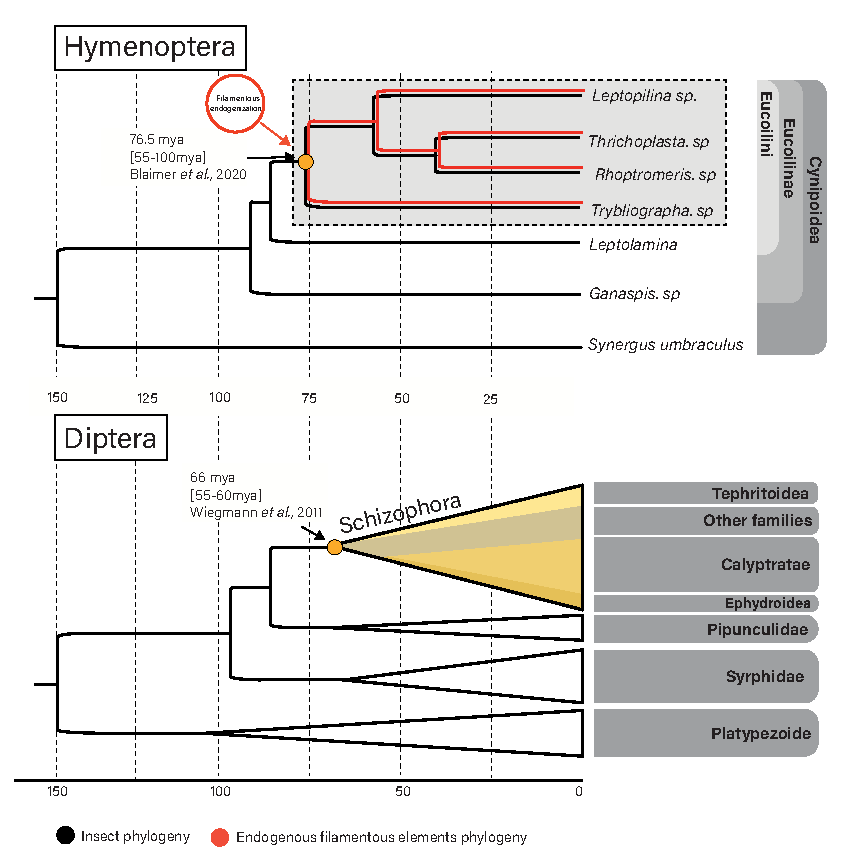
\includegraphics[width=\linewidth,height=\textheight,keepaspectratio]{PhD-master/figures/Schizophora_cynipids_virus_phylogeny.pdf}\centering
\caption[Paper3:Schizophora and Eucoilini datation phylogenies]{\textbf{Phylogenetic host and filamentous EVEs trees}. Black branches correspond to Hymenoptera (up) or Diptera (bottom) branches, while red branches correspond to filamentous EVEs branches. Trees were reconstructed using the following sources : \citep{blaimer_comprehensive_2020} for Hymenoptera datatation, and \citep{wiegmann_episodic_2011} for the Diptera datation. The endogenous filamentous virus phylogeny was inferred with the concatenation of the  16 endogenous filamentous viral elements shared within all Eucoilini).}
\label{figure:Schizophora_Eucoilini_virus_phylogeny}

\end{figure}

\subsection{Filamentoviridae originated between the Carboniferous and the Triassic around 297 mya}

To infer the evolutionary history of \textit{Naldaviricetes}, we calibrated the phylogeny using two points. The first included the documented nudiviral domestication event that happened in the common ancestor of the Microgastroids 100 million years ago \citep{whitfield_virus_2003, bezier_bracovirus_2008, murphy_phylogeny_2008}. The second comprised estimations of the common ancestor of the 6 Eucoilini species that captured the filamentous genes around 75 million years ago \citep{blaimer_comprehensive_2020}. These calibrations revealed that Filamentoviridae might have had their beginnings between 241 and 352 million years ago (\figurename{\ref{figure:Cynipoidea_dsDNA_datation_plot}}). On the other hand, this analysis also allowed to estimate the divergence time of other \textit{Naldaviricetes} families. Thus, we estimated the divergence of the \textit{Hytrosaviridae} (between 24 and 310 mya), the \textit{Baculoviridae} (between 164 and 328 million years ago, and the \textit{Nudiviridae} (between 247 and 346 mya).


\begin{figure}[!htpbt]
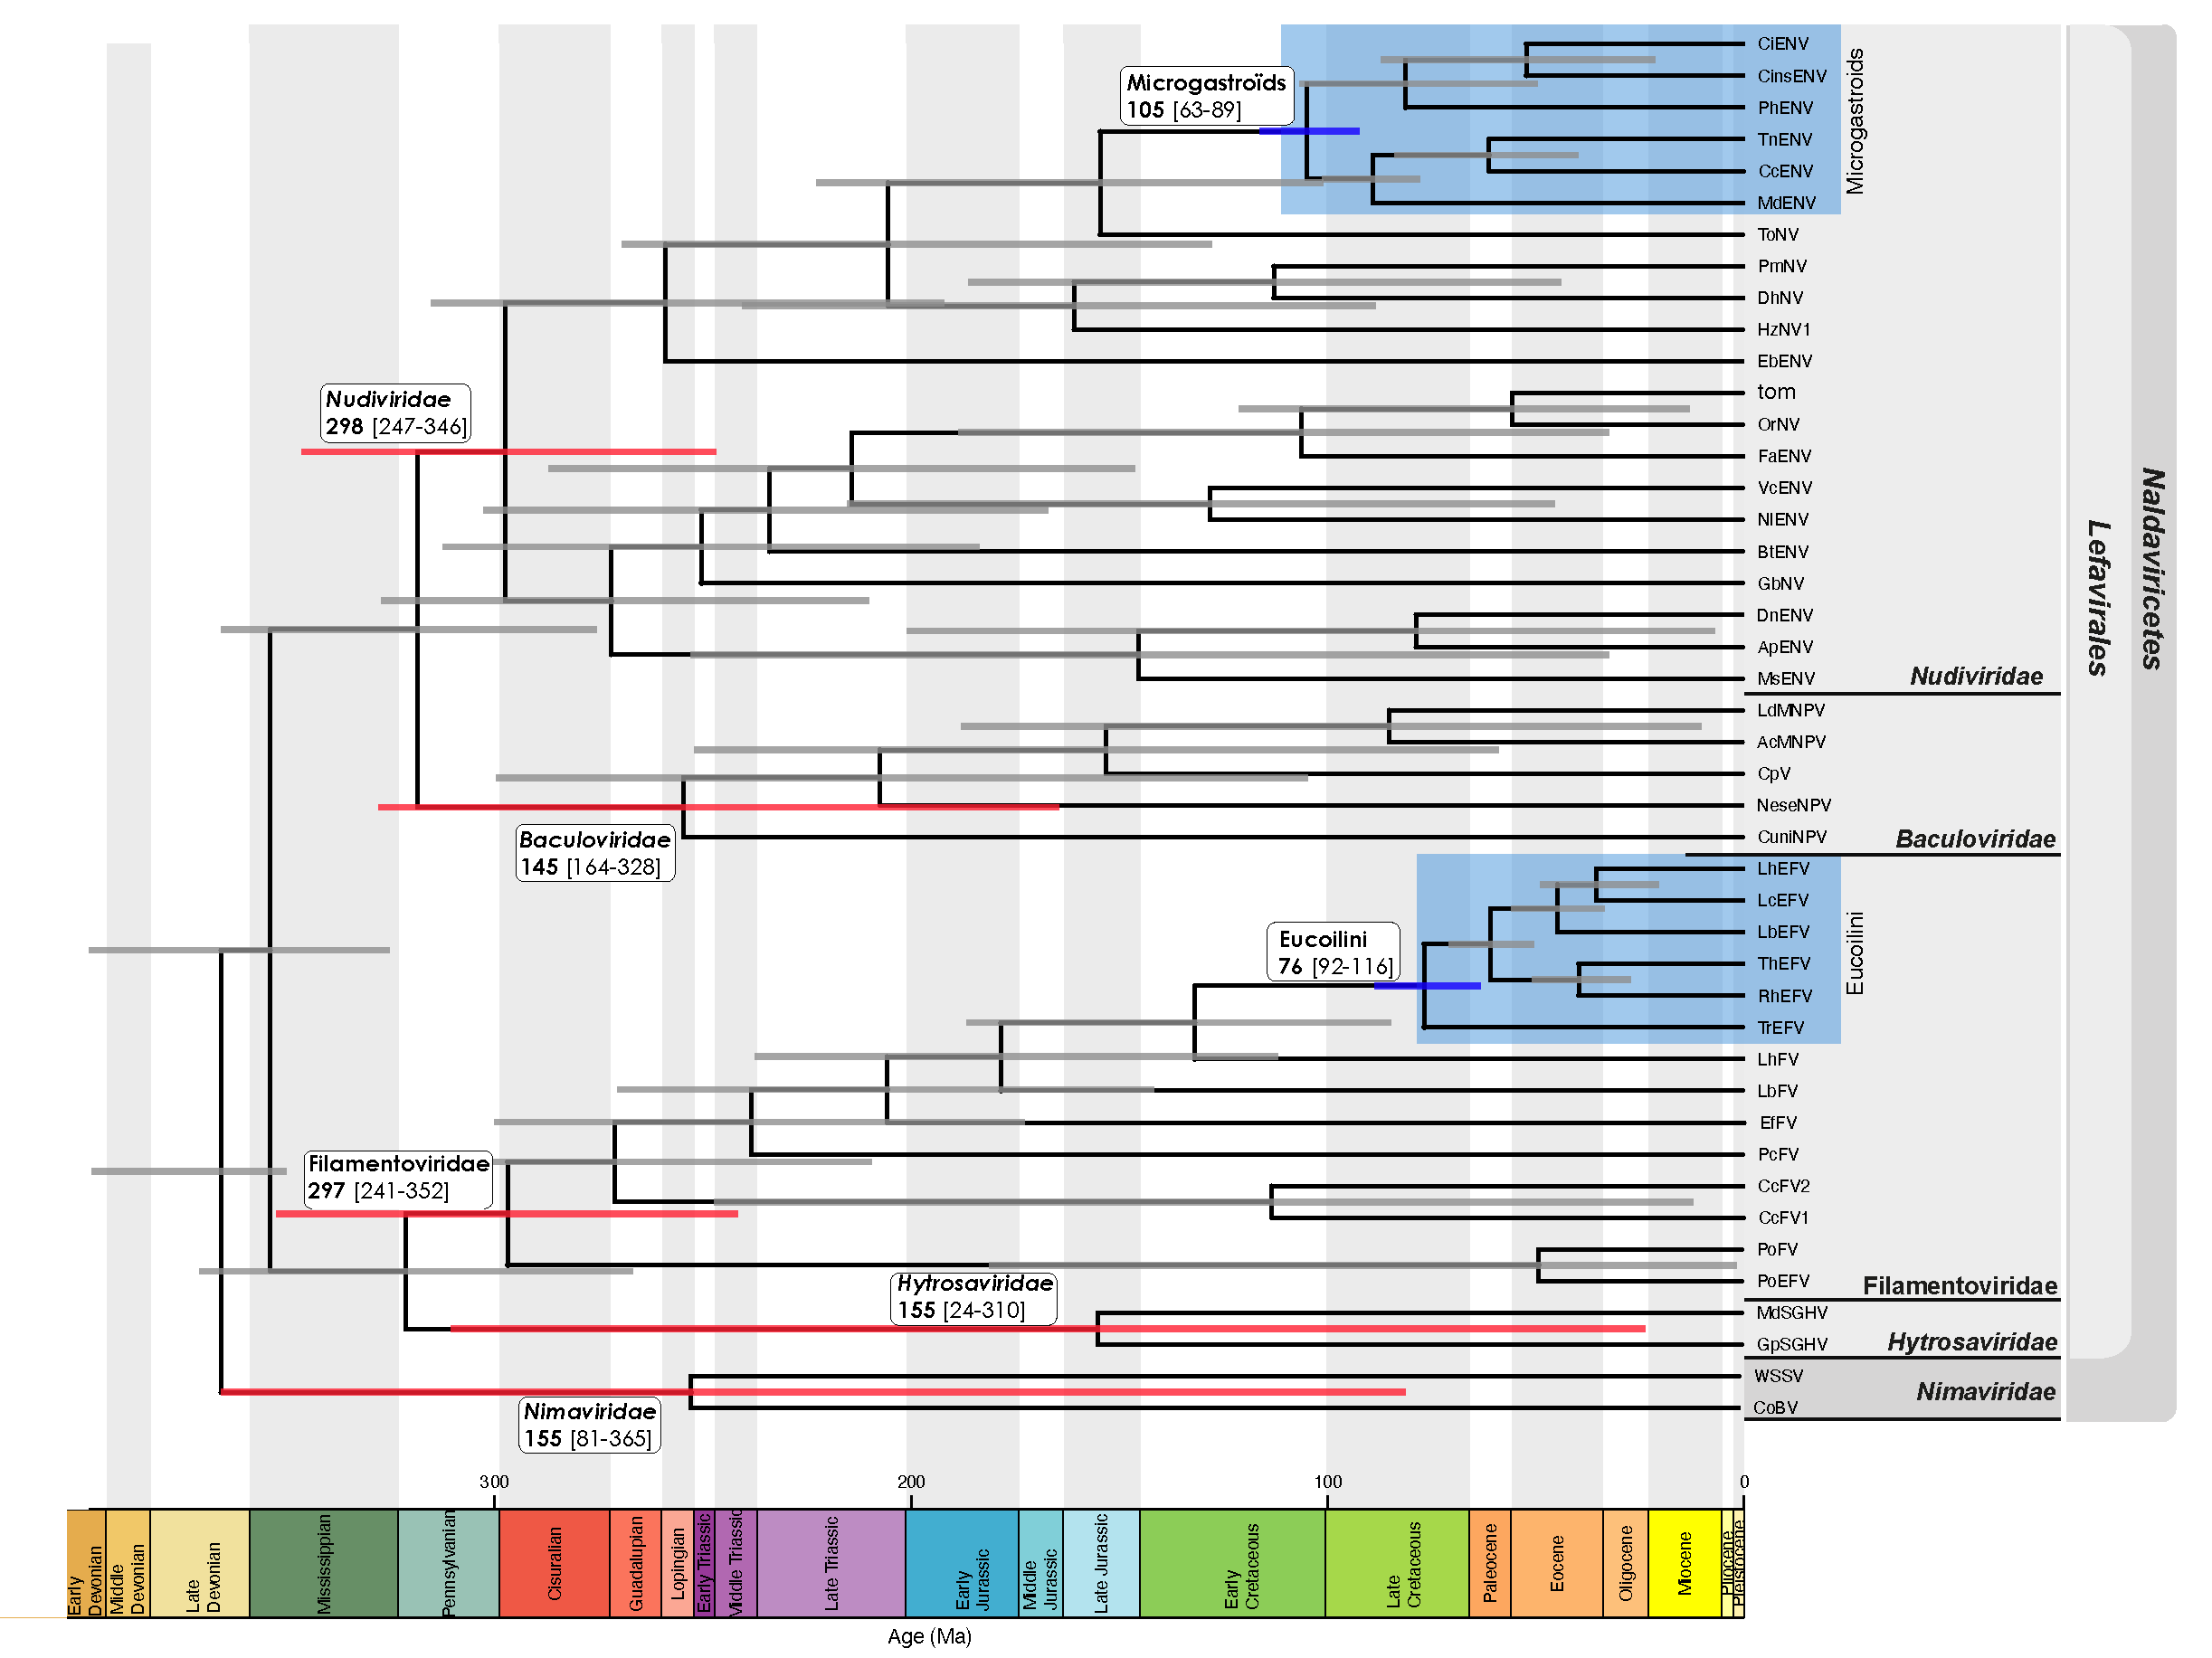
\includegraphics[width=\linewidth,height=\textheight,keepaspectratio]{PhD-master/figures/Cynipoidea_dsDNA_datation_plot.pdf}\centering
\caption[Paper3:\textit{Naldaviricetes} dated phylogeny including Eucoilini]{\textbf{Phylogenetic tree datation inference of the \textit{Naldaviricetes} clade}. Green posterior distributions represent date estimations for endogenous events, while red posterior distributions represent date estimations for the \textit{Naldaviricetes} family.}
\label{figure:Cynipoidea_dsDNA_datation_plot}
\end{figure}


\section{Discussion}

In this article, we showed two independent filamentous virus endogenization events in 6 Eucoilini species including \textit{L.clavipes}, \textit{L.heterotoma}, \textit{L.boulardi}, \textit{Trichoplasta}, \textit{Rhoptromeris} and \textit{Trybliographa}, but not in the \textit{Leptolamina} genome which is the most basal species of the Eucoilini tribe. One event occurred in the common ancestor of 6 Eucoilini species around 75 million years ago and concerned at least 18 filamentous EVEs. A secondary independent event including 9 filamentous EVEs concerned the \textit{Rhoptromeris} species. We will respectively call these two independent endogenization events : \textit{ancestral event} and \textit{recent event} in the following discussion section. Finally, these results allowed us to calibrate the phylogeny of the filamentous virus from which these EVEs derive. A bayesian analysis estimated that the putative Filamentoviridae family emerged somewhere between the Carboniferous and Permian periods around 297 million years ago.  \\

To date, it has been determined that all \textit{Leptopilina} species tested produce VLPs in their venom gland \citep{rizki_parasitoid_1990, morales_biogenesis_2005}.  These particles are formed during the pupal stage and kept in the venom gland's reservoir. Females inject not only their egg(s) but also some VLPs into their \textit{Drosophila} hosts during oviposition. Conceptually, VLPs are comparable to liposomes that would contain virulence proteins. VLPs then allow the wasp to transport these proteins to the immune cells of Drosophila \citep{colinet_convergent_2007}. The virulence proteins produce significant morphological changes in the lamellocytes, preventing them from launching an effective immune response against the parasitoid egg \citep{colinet_convergent_2007}. It has been shown previously that the present-day VLPs arose through endogenization and domestication of 13 ancient filamentous viral genes (Di Giovanni et al., 2020). Using genes of both viral and eukaryotic origin, these "hybrid" structures now enable the delivery of eukaryotic virulence proteins to the \textit{Drosophila} immune cells, thus protecting the developing wasp from encapsulation. \\


Our analysis indicate that this endogenization process is not limited to \textit{Leptopilina} species, but instead affects nearly all Eucoilini species that inherited these genes from their common ancestor, which raises the question of the function of these filamentous EVEs outside of the \textit{Leptopilina} species.

All Eucoilinae are solitary koinobiont endoparasitoids that prey on larvae of the Cyclorrhapha Diptera suborder.
More specifically, while  \textit{Leptopilina} species are known to infect Drosophilidae, \textit{Rhoptromeris} genus are known to infect Chloropidae flies, \textit{Trybliographa} to infects Anthomyiidae flies, and \textit{Thrichoplasta} to infects Drosophilidae, Muscidae, and Lonchaeidae files. All thes especies are distributed worldwide except for some of them not found in Neotropical regions \citep{nordlander_identities_1982}. More generaly, the Eucoilini species are descended from the extraordinarily diversified Figitidae family, of which the subfamily Eucoilinae (83 genera, 987 species) is by far the most species-rich, accounting for around 33\% of the Figitidae genus \citep{fontal-cazalla_phylogeny_2002,ronquist_phylogeny_1995,ronquist_phylogeny_2015}.


It has been demonstrated in \textit{Leptopilina} that the filementous EVEs are significantly expressed in the female venom gland during the early part of the pupal stage, when VLP synthesis starts (Di Giovanni et al., 2020). On this basis, it is possible to postulate that all Eucoilini species harboring these EVEs as well would exhibit the same pattern and produce VLPs. As expected for genes involved in the production of fitness-related structures like VLPs, we discovered that all 18 EVEs in Eucoilini species were subject to intense purifying selection (\figurename{\ref{figure:dNdS_position_plot}}). If only a subset of Eucoilini species produced these VLPs, we would anticipate these EVEs to be deteriorated by selective drift. However, after more than 75 million years of evolution, all of these genes are still intact in these species. In addition, even if we lack information regarding transcription assay in the Eucoilini species, we may have another argument to support our claim. Indeed, in her PhD, Nabila Kacem Haddj El Mrabet described in 1999 discovered VLPs in the venom gland of \textit{Trybliographa rapae} (\figurename{\ref{figure:Microscopy_Lboulardi_Trybliographa}}). These results show that VLPs are also produced by the one of the most basal species of the Eucoilini, further supporting that the other species might also produce VLPs derived from the filamentous genes. 

\begin{figure}[!htpbt]
\includegraphics[width=\linewidth,height=\textheight,keepaspectratio]{PhD-master/figures/Microscopy_Lboulardi_Trybliographa.pdf}\centering
\caption[Paper3:[Electronic microscopy of \textit{L.boulardi} and \textit{T.rapae} VLPs]{Electronic microscopy pictures of VLPs produced in the venom gland of \textit{Lepoptilina boulardi} (A) and \textit{Trybliographa rapae} (B) from \cite{di_giovanni_behavior-manipulating_2020} and D.Poinsot and K.Haddj E PhD 1999 respectively.}
\label{figure:Microscopy_Lboulardi_Trybliographa}
\end{figure}

If this hypothesis is accurate, we can speculate about novel functions brought by our analysis that might be involved in the VLPs productions. 

One new important function came from the filamentous \textit{lef-5} EVE. The \textit{lef-5} is an important protein in baculovirus replication, where it acts as a transcription initiation factor \citep{su_autographa_2011}. In the AcMNPV genome, a knockout of the \textit{lef-5} gene revealed that it was required for productive infection \citep{su_autographa_2011}. On the other hand, the polydnavirus  production in \textit{M.demolitor} seems to require a \textit{lef-5} while it is absent in \textit{C.vestalis} or \textit{C.inanitus} \citep{burke_common_2019}. In other VLP-producing wasps (\textit{V.canescens} and \textit{F.arisanus}), lef5 has also been identified. This may suggest that the presence of \textit{lef-5} is not strictly required for the production of polydnaviruses, but it seems to be the case for VLP production. Our analysis revealed that this gene was evolving under purifying selection, suggesting its important role in parasitoid biology. Taken together, these results suggest that Eucoilini retained the filamentous-like RNA polymerase initiation factor (\textit{lef-5}) that likely mediates transcription of several filamentous-like structural components that form VLPs virions. Likewise, we found in all Eucoilini species the presence of the filamentous RNA polymerase complex genes (\textit{lef-4}, \textit{lef-9} and \textit{lef-8}). Thus, jointly with the initiation factor (\textit{lef-5}), this strongly suggests that all filamentous-carrying wasps likely have the genes necessary to form a complete RNA polymerase complex. Furthermore, the presence of a filamentous-like DNA \textit{helicase} and a \textit{DNA polymerase} suggests that a portion of the ancestral viral DNA replication machinery is still functional in the Eucoilini species. Indeed, previous work identified that 10 out of 13 filamentous EVEs were amplified during VLP production, probably using the filamentous viral machinery (Di Giovanni et al., 2020). This feature is quite different from other polydnavirus and VLPs systems found in Ichneumnoidea where in \textit{V.canescens, F.arisanus} and Microgastroïds, the \textit{DNA polymerase} is consistently missing from nudivirus-derived endogenous viruses \citep{burke_common_2019,petersen_naked_2022}.

Only one gene (LbFVorf44) was uniquely found in the \textit{L.boulardi} genome in multiple copy (n=37), and one of these copy was found within the same scaffold of another EVE, suggesting this gene was brought during the same event and was then followed by many duplication events since no paralogs could be found within the LbFV closely related donor genome. Many copies presented an intact open reading frame and evolved under purifying selection. In others domesticated models such as is \textit{M.demolitor}, multiple genes have shown many tandem duplications of domesticated nudiviral such as the \textit{odv-e66} present in multiple copies both in \textit{M.demolitor} and \textit{C.congregate} \citep{gauthier_chromosomal_2021}. One paper speculated that such duplication might be adaptive, since the \textit{odv-e66} encodes a viral chondroitinase that digests the gut's peritrophic membrane, allowing primary infection \citep{gauthier_chromosomal_2021}. The large gene family expansion could therefore have contributed to the wasp's adaptation, possibly in a gene for gene coevolutionary framework \citep{gauthier_chromosomal_2021}. 

Finally, we were able to hypothesize a function for the  LbFVorf10 gene, which is also present in the LbFV genome. Interestingly, this gene showed a 3D structural homology with a Glycoprotein containing a Zinc finger domain found in the ssRNA(-) Hantavirus (\textit{Bunyaviridae}) protein (\figurename{\ref{table:ORF_functions}}). Despite the total absence of sequence conservation, the complex 3D fold was significantly similar between Hantavirus glycoprotein 3D structure and the LbFVorf10  (HHpred evalue =9.5e-7). This means that analogue function could be involved. Hantavirus particles are lipid-enveloped and have a surface lattice composed of tetragonal spikes made from two glycoproteins, Gn and Gc. The glycoprotein shell of Hantavirus is responsible for coordinating all the steps required for viral entry and is the primary target of the antibody-mediated immune response \citep{guardado-calvo_surface_2021}. One could therefore speculate that such gene in filamentous genomes as well as in the VLPs might be involved in facilitating the entry of viral structures into host cells by binding to cell surface receptors. It could also be responsible for triggering an immune response in the host, which helps protect the host from infection \citep{guardado-calvo_surface_2021}.\\

According to prior estimates, the common ancestor of the 6 Eucoilini species that domesticated the ancestral filamentovirus lived in the Cretaceous approximately 75 million years ago [55mya-100mya] \citep{blaimer_comprehensive_2020}. Besides, the most species-rich group within the Eucoilini Cyclorrhapha hosts is undeniably Schizophora, which accounts for one-third of fly diversity within Cyclorrhapha, with over 55,000 known species \citep{bayless_beyond_2021}. It has been estimated that this group of flies diversified rapidly 55 to 60 million years ago (\figurename{\ref{figure:Schizophora_Eucoilini_virus_phylogeny}}) \citep{bayless_beyond_2021}. On the other hand, Eucoilini are also highly diverse \citep{fontal-cazalla_phylogeny_2002,ronquist_phylogeny_1995}.

Given the uncertainty around the average dating values, the diversification of the Schizophora hosts would have occurred around the same age as the spread of Eucoilini wasps. (\figurename{\ref{figure:Schizophora_Eucoilini_virus_phylogeny}}) \citep{blaimer_comprehensive_2020}). Consequently, one could hypothesize that this co-occurrence is likely related to the new benefit conferred by the accidental filamentous endogenization that occurred at the same age. This would have enabled the formation of VLPs in Eucoilini wasps, allowing them to better colonize and adapt to new Schizophora hosts during the early radiation of the group. Similar scenarios have been proposed to account for the radiation observed in the Microgastroid complex's after the   domestication of an ancestral nudivirus, 100 million years ago \citep{whitfield_virus_2003, bezier_bracovirus_2008}.

Interestingly, we also described a new endogenization event involving 9 filamentous genes in the \textit{Roptromeris} genome, which would have occurred after the ancestral event in the Eucoilini. Some of these genes displayed evidence of pseudogenization, indicating that enough time has passed for accumulating enough mutations for genes to degenerate. 

Three of them were redundant with a gene acquired after the initial ancestral event. These 3 genes exhibited a complete open reading frame, indicating that they may be functioning. 

More strikingly, we also detected a possible replacement of a viral gene by another homologous viral gene. Indeed, the LbFVorf10 gene is present in all Eucoilini; however, for Leptopilina, \textit{Trybliographa}, and \textit{Trhichoplasta}, it arose from the first event, but for \textit{Rhoptromeris}, it originated from the second. If these results are accurate, the LbFVorf10 EVE introduced by this recent event has replaced the LbFVorf10 EVE introduced by the ancestral event in the \textit{Rhoptromeris} genome. Besides,  according to 3D structural homology, this gene has a structural homology with a Hantavirus protein involved in facilitating the virion entry into host cells by attaching to cell surface receptors. Therefore, we can speculate that the replacement of this gene in \textit{Rhoptromeris} may have facilitated the effective entry of VLPs into host cells.  

Finally, using the information provided by the ancestor endogenization event in Eucoilini (filamentous virus - VLPs) and Microgastroid (nudivirus-polydnavirus), we were able to calibrate the \textit{Naldaviricetes} phylogeny in which the two donor viruses belongs.  

These calibrations revealed that Filamentoviridae might have originated between 241 and 352 million years ago (median = 297mya)(\figurename{\ref{figure:Cynipoidea_dsDNA_datation_plot}}), coinciding with the time when the Hymenoptera began to diversify between the Carboniferous and the Triassic (239-329 million years ago) \citep{peters_evolutionary_2017}. These results are consistent with a recent study that suggested that Filamentoviridae were preferentially infecting Hymenoptera species (\hyperref[sec:chap2]{chapitre 2}:\textit{in prep}).   More specifically, it appears that Filamentoviridae is more closely associated with parasitoids wasps, whose most diverse parasitoid wasp lineages (i.e., Ceraphronoidea, Ichneumonoidea, and Proctotrupomorpha) underwent a remarkable radiation 195 to 266 million years ago, quite after the Filamentoviridae establishment. 

Such a long-term association surely opened the door to many genetic exchanges between filamentous viruses and their hosts, as it can be seen for nudiviruses in many arthropod species (\figurename{\ref{figure:Host_virus_phylogeny_last}}). For instance, two endoparasitoid of the Ichneumonidea family : \textit{Dolichomitus sp} and \textit{Cotesia vestalis} \citep{burke_endogenization_2020} presented evidence for endogenization of filamentous-related EVEs and an endoparasitoid wasp from the Platygastridae family \textit{P.orseoliae}, also presented evidences of domesticated filamentous EVEs (\figurename{\ref{figure:Host_virus_phylogeny_last}}). Additionally, a recent data mining analyze on all Hymenoptera species available in public databases revealed the presence of filamentous EVEs in more than 10\% of Hymenoptera species (Bguinet et al., \textit{in prep}). Interestingly, while the number of filamentous EVEs were much less than in Hymenoptera, these results also point out the presence of filamentous EVEs in other order species : 3\% in Lepidoptera assemblies and less than 1\% of Diptera assemblies suggesting that these genes might have been acquired through parasitism by hymenopteran infected by such viruses \citep{muller_genome-wide_2021}. 

Given the high prevalence of filamentous EVEs within this Hymenoptera samples, we could anticipate an explosion in the detection of new filamentous species as genome sequencing increases. In addition, these data indicate that recipient genomes have many opportunities to select and domesticate the integrated viral machinery if such opportunity gives a selective advantage. 


\section{Materials and methods}


\subsection{41 \textit{Cynipoidea} specimens extractions}

All extractions were performed with the NucleoSpin Tissue Macherey kit. 31/41 Cynipoidea specimens were extracted with the whole body, while 10/41 were extracted with the abdomen in order to keep the upper body for morphological identification (when only one individual was available). Consequently, we adapted the volumes according to the selected tissues, in the following we call the volumes for the full bodies "c", and the abdomens "a". The bodies or abdomens were manually crushed with a piston in a 1.5Ml eppendorf tube with proteinase K (c:180$\micro$L / a:60$\micro$L) and T1 buffer (c:25$\micro$L / a:8$\micro$L) and then incubated at 56 °C for 3h. The lysates were then mixed and buffer B3 (c:200$\micro$L / a:70$\micro$L) was added and incubated at 70 °C for 10 min. The whole solution was then bound to a silica column with the addition of ethanol (a :210$\micro$L / c:70$\micro$L) followed by a 1-minute centrifugation step at 11000G. The columns were then washed with the addition of buffer BW (a:500$\micro$L / c:250$\micro$L), followed by a 1-minute centrifugation at 11000G, then the addition of buffer B5 (a:600$\micro$L / c:300$\micro$L) followed by a 1-minute centrifugation at 11000G. The DNA was then eluted in 20$\micro$L of TE. 

\subsection{PCR amplification of ORF96}
Based on the sequences of \textit{L. boulardi}, \textit{L.heterotoma} and \textit{L. clavipes}, we used the same LbFV\_ORF96 primers as in \cite{di_giovanni_behavior-manipulating_2020} (ATTGGTGAAATTCAATCGTC and TCATTCATTCGCAATAATTGTG). They amplified a 411bp internal fragment of the coding sequence. PCR reaction was performed in a 50$\micro$L volume containing 10$\micro$M primers, 10mM dNTPs, and 0.5uL of Taq DNA polymerase with the following cycling conditions : 95 C 30",48 C 30", 72 C 60" (40 cycles). The CO1 marker was correctly amplified in 33 out of 41 specimens, indicating that extraction was satisfying, at least for these specimens. Finally, because we had sometimes several specimens per species, all species but two could be analyzed with at least one specimen.

\subsection{Genome sampling, assembly quality check}
The DNA of single female was extracted using the same protocol from \textit{Rhoptromeris}, \textit{Trybliographa},\textit{Leptolamina} and \textit{Thrichoplasta}. TruSeq Nano DNA (350) Illumina libraries were built and sequenced with 30 Gb per sample 60M(R1+R2) at Macrogen (Amsterdam, Netherlands). The paired-end reads (2x150bp) were cleared from duplicates using SuperDeduper v1.3.0 \citep{petersen_super_2015}  (-f nodup), and quality trimmed using Fastp v0.22.0 (--cut\_tail --length\_required 100 --correction). The assembly was done using Megahit v1.2.9 \citep{li_megahit_2015} (--kmin-1pass), a scaffolding step was done using SOAPdenovo-fusion (-D -s) and we obtained a scaffolded homozygous genome assembly using the Redundans pipeline \citep{pryszcz_redundans_2016} (default parameters). The genome assembly quality check was done using the BUSCO pipeline v 5.3.0  \citep{simao_busco_2015} (-m genome) on both Hymenoptera and Arthropoda databases, and assembly statistics were computed using Quast \citep{gurevich_quast_2013} (default parameters) (see genome statistics on Github: 
\href{https://github.com/BenjaminGuinet/PhD_defense/blob/main/Supplementary_paper3/Cynipoidea_genomic_assembly_quality.xlsx}{Cynipoidea\_genomic\_assembly\_quality.xlsx}).

\subsection{LbFV-like ORF homology sequence research}

We screened all \textit{Cynipoidea} genomes for the presence of ORFs from LbFV-like virus genomes. The sequence homology search was performed using the Mmseqs2 search algorithm \citep{steinegger_mmseqs2_2017} (evalue max = 0.001 -s 7), using as queries all the  predicted proteins from the \textit{Naldaviricetes}  (see details in (\hyperref[sec:chap2]{chapitre 2}:\textit{in prep})) and as database the 11 Cynipoidea genomes. In order to infer the phylogenetic relationships between the endogenized sequences and free-living viruses, we first sought to gather the homologous ORFs between them. To do this, we performed a blastp between all ORFs with the mmseqs2 search algorithm (min bit = 50, min evalue = 1e-04). We then formed clusters between all genes that had at least one homology with one of the members, following the same pipeline used in (\hyperref[sec:chap2]{chapitre 2}:\textit{in prep}). 

%To ensure that the clustering step did not assemble several non-homologous proteins, we counted the number of loci present in more than two copies among the clusters. The clusters that had more than 4 duplicated copies and where more than 70\% of the loci were duplicated were reanalyzed using a more stringent clustering (min bit score = 55, min evalue = 1e-06). These reassembled clusters have the assignment 'redefined'. 

%Based on the homologies between ORFs, clusters of homologous sequences were established. Following this, we carried out a second, more sensitive clustering process. As a result, we created profiles for each of the clusters (HMMER profile v3.3.2). Then, HMMER search was used to do a HMMER search between all cluster profiles and the initial database (all ORFs). We integrated the cluster from which the ORF originated with the cluster from which the profile derived if one or more ORFs had convincing hits (e-value max = 9e-05) with one or more clusters. In this step, homologous ORFs that were not assembled in the same cluster because of the stringency were combined.

\subsection{Endogenization arguments}

A way to rule out contaminating scaffolds was to look for the presence of insects genes along the scaffolds containing candidate EVEs, assuming that the presence of several insect genes in a viral scaffold is unlikely (except for specific giant viruses or specific insect genes such as apoptotic genes). Eukaryotic genes research was made using the Metaeuk easy-predict workflow \citep{levy_karin_metaeuksensitive_2020} (default parameters) followed by the taxtocontig workflow that allows to assign taxonomic labels to the predicted MetaEuk proteins. For each contig, we adopted a majority voting strategy among the taxonomically labeled protein to assign taxonomy to the contig. As an example, a contig was tagged as "Eukaryota origin" if at least 50\% of the labels assigned to the encoded proteins were "Eukaryota". 

We were also used the presence of transposable elements in contigs as a marker of its eukaryotic nature. Indeed, so far, very few viral genomes have been shown to contain transportable elements \citep{miller_virus_1982,gilbert_population_2014,gilbert_continuous_2016,gilbert_viruses_2017,loiseau_wide_2020}. Thus, the probability for a viral EVE to be flanked by a TE is low, even more so if the number of flanking TEs is greater than 1. These results suggest that TE insertions rarely reach high frequencies in viral populations due to the fact that the majority of endogenizations of TEs in viral genomes are deleterious and are quickly eliminated by selection \citep{gilbert_continuous_2016, gilbert_viruses_2017}.
We thus looked for TE sequence homology in the scaffolds harboring candidate EVEs (see details in M.M Transposable elements' detection and analysis) and identified the scaffolds presenting one or more TE. 

\subsection{LbFV-like EVEs phylogenies and Event assignations}

To reconstruct the phylogenetic history of each EVE originating from filamentous viruses (n=25), we first aligned the protein sequences using ClustalO  (v1.2.4)\citep{sievers_fast_2011} and then inferred the phylogenies using Iqtree (v2.1.2) \citep{minh_corrigendum_2020} (options :m MFP -alrt 5000 -bb 5000). The phylogenetic tree was then used to infer endogenization events involving Eucoilini species. It is expected that such events will be represented by a monophyletic clade of related wasp species nested within a clade of filamentous viruses. Within each phylogenetic tree, we grouped all Eucoilini wasp species into a single event, if they formed a monophyletic clade with a bootstrap score greater than 80. 

\subsection{Aggregation of different EVEs in a single endogenization event}

In case multiple EVEs arrived together into the ancestral wasp genome, we expect to find signs of shared synteny between descendant species. To do this, we conducted the equivalent of an all vs all TblastX (Mmseqs2 search --search-type 4, max Evalue =1e-07) between all the candidate loci within a putative event (deduced from the phylogenetic inference), and then looked for hits (HSPs) between homologous EVEs around the insertions. Because it is possible to find homology between two genomic regions that does not correspond to an orthology relationship, for example because of the presence of conserved domains, we had to define a threshold to identify with confidence the orthology signal. We therefore conducted simulations to define this value, based on the well assembled genome of \textit{Cotesia congregata} (GCA\_905319865.3) by simply performing the same all vs all blast analysis against itself (as if the two species considered had the same genome). Based on this, we defined two types of simulated EVEs, (i) independently endogenized EVEs in the genomes of the two "species". This is simply simulated by randomly selecting two different regions in the genomes, and (ii) a shared  simulated EVE that was acquired by their common "ancestor". This is simulated by selecting  the same random genomic location in both "genomes". We then counted the total length of the HSPs found around the simulated insertions all along the corresponding scaffold (i and ii). As the result will obviously depend on scaffold length, we performed these simulations on several scaffold lengths (100000000bp, 10000000bp, 1000000bp, 100000bp and 10000bp). 
We conducted 500 simulations in each scenario, and we measured the cumulative length of homologous sequences, where homologous sequences are defined by sequences having a bit score $>50$. We then defined a threshold for each windows size in order to minimize for the false-positive (FP) and maximize true-positifs (TP)  (thresholds 100000000bp = 172737bp (FP = 0.012, TP= 0.922); 10000000bp = 74262 bp (FP= 0.012, TP=0.878) ; 1000000bp = 21000 bp (FP=0.014, TP=0.28); 100000bp = 1332 bp (FP= 0.012 TP= 0.198) and  10000bp = 180 bp (FP= 0.008, TP= 0.208)). 
This way, the EVEs could be "aggregated" into single events. 

\subsection{Filamentoviridae time estimation}

To estimate the timescale of filamentous virus evolution, n=50 clusters containing at least four homologous sequences were subjected to a molecular clock analysis. We omitted the AmFV and DoFV sequences from the analysis because of the uncertainty in the correct positions for AmFV or because it was unclear whether DoFV scaffolds belonged to free-living or endogenous entities. We time-calibrated the previously inferred  \textit{Naldaviricetes} tree using a Bayesian approach on RevBayes 1.1.1 \cite{hohna_probabilistic_2014}. Evaluation of the phylogenetic likelihood being the most expensive operation when calculating the posterior density, we decided to use the method developed in \cite{szollosi_relative_2020} to reduce computational cost and approximate the phylogenetic likelihood using a two-step approach. In the first step, the posterior distribution of branch lengths measured in expected number of substitutions is obtained for the fixed unrooted topology of using a standard MCMC analysis (100,000 iterations, 3 chains, 5000 burn-in, tuningInterval=200). The obtained posterior distribution was then used to calculate the posterior mean and posterior variance of the branch length for each branch of the unrooted topology. In the second step, we date the phylogeny using a relaxed clock model and calibrations (500,000 iterations, 4 chains, 5000 burn-in, tuningInterval=200). In order to calibrate the nodes, we relied on two independent single endogenization events that occurred approximately 100 million years ago in Microgastroids and 75 million years ago in the common ancestor of nearly all Eucoilini species (except \textit{Leptolamina})\citep{blaimer_comprehensive_2020}. Consequently, following a divergence time estimate for Microgastoids, we specified the following truncated normal prior distribution based on fossil estimates from the paper \citep{murphy_phylogeny_2008} (node 1 : dnNormal(mean=87, sd=7, min=82, max=92), node 2 : dnNormal(mean=103.38, sd=7, min=98.97, max=107.79).
Concerning node calibration within the Eucoilini clade, we modelled the previously posterior bayesian prediction based on fossils of \citep{blaimer_comprehensive_2020} to calibrate the same node in our analysis and consider the estimations (node3 : dnNormal(mean=74.1,  sd=8.63, min=55.25, max=91.4), node4 : dnNormal(mean=55.46, sd=7.95, min=39.86, max=71.67), node5 : dnNormal(mean=40.654, sd=8.21, min=11.19, max=81.07) and node6 : dnNormal(mean=38.86, sd=8.41, min=22.3, max=55.4). For 1,5 million  generations on 2 independent runes with 42 chains, Markov chain Monte Carlo (MCMC) analyses were conducted by sampling every 10,000th generation. Tracer was used to ensure that all effective sample sizes for MCMC runs were greater than 200.

\section{Supplementary figures}


\begin{figure}[!htpbt]
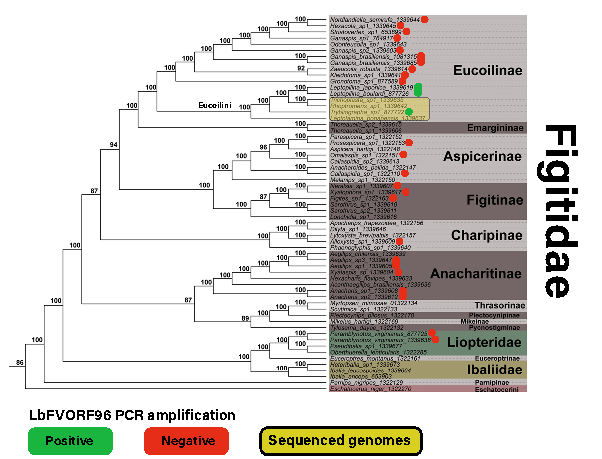
\includegraphics[width=\linewidth,height=\textheight,keepaspectratio]{PhD-master/figures/Figitidae_PCR_genomes.pdf}\centering
\caption[Paper3:Figitidae phylogenetic tree with all sampled species]{\textbf{Figitidae phylogenetic tree with all sampled species}. The figure is modified from the previous work of \cite{blaimer_comprehensive_2020}. Positive PCR amplification of ORF96 for each genus is displayed in green, while negative in red. This only concerns genus in the phylogeny, it does not mean the specific taxa as been tested. To see the specific species tested, please refer to the (\figurename{\ref{figure:Electrophoresis_ORF96}}). Genus that were newly sequenced and assembled are in yellow box, this includes \textit{Leptolamina}, \textit{Trybliographa}, \textit{Thrichoplasta} and \textit{Rhoptromeris}.}
\label{figure:Figitidae_diversity}
\end{figure}


\begin{figure}[!htpbt]
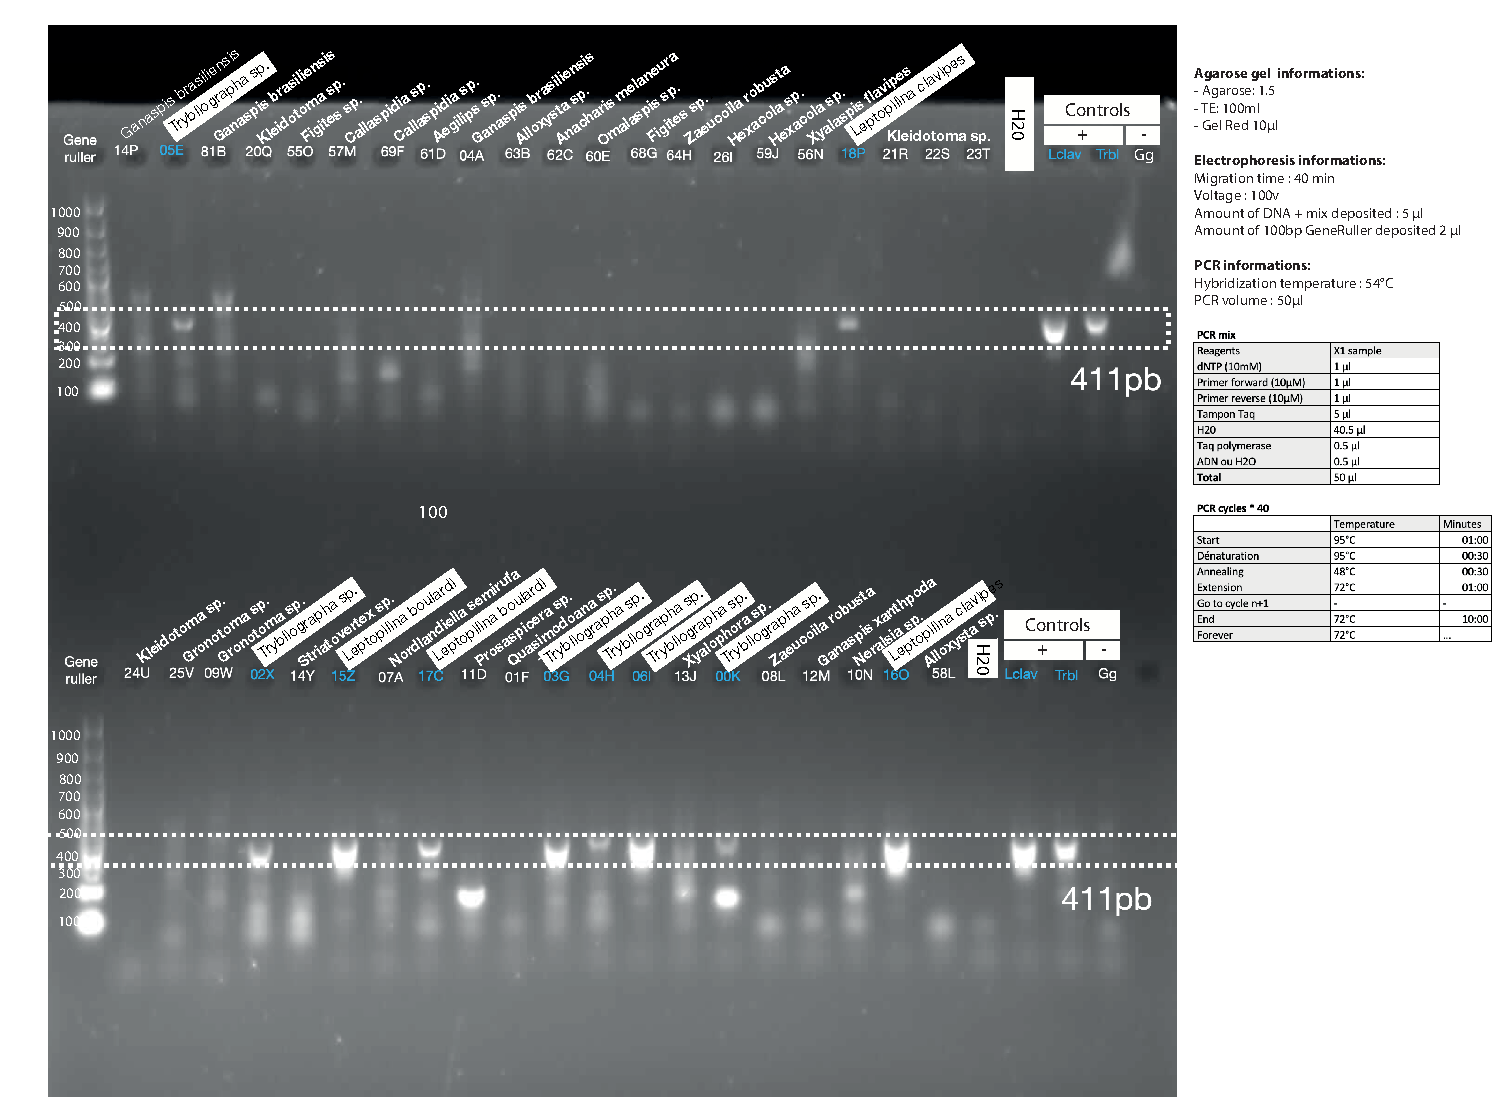
\includegraphics[width=\linewidth,height=\textheight,keepaspectratio]{PhD-master/figures/Electrophoresis_ORF96.jpg}\centering
\caption[Paper3:ORF96 PCR results on Figitidae species]{\textbf{ORF96 PCR results}. Positive PCR amplification of ORF96 is displayed by a blue number and a white box. The expected ORF96 amplicon size was 411bp and is delimited with the doted white rectangles.}
\label{figure:Electrophoresis_ORF96}
\end{figure}


\begin{figure}[!htpbt]
\includegraphics[width=\linewidth,height=\textheight,keepaspectratio]{PhD-master/figures/ALL_cunipids_species_Cov_GC.jpg}\centering
\caption[Paper3:Eucoilini COV/GC scaffold ditributions]{\textbf{Coverage and G+C\% content of scaffold harboring filamentous EVEs}.  General features of scaffolds containing single copy universal arthropod genes (BUSCO gene set, in grey). Scaffolds containing filamentous virally derived loci are in blue. The size of the dots corresponds to the number of candidate EVEs inside the scaffold. The dots circled in black correspond to scaffolds that contain one or more eukaryotic genes and/or one or more repeat elements. (A) \textit{L. boulardi} ;  (B) \textit{L. clavipes} ; (C) L. heterotoma ; (D) \textit{Rhoptromeris sp} ; (E) \textit{Trybliographa} ; (F) \textit{Thrichoplasta}.}
\label{figure:ALL_cunipids_species_Cov_GC}
\end{figure}

\begin{figure}[!htpbt]
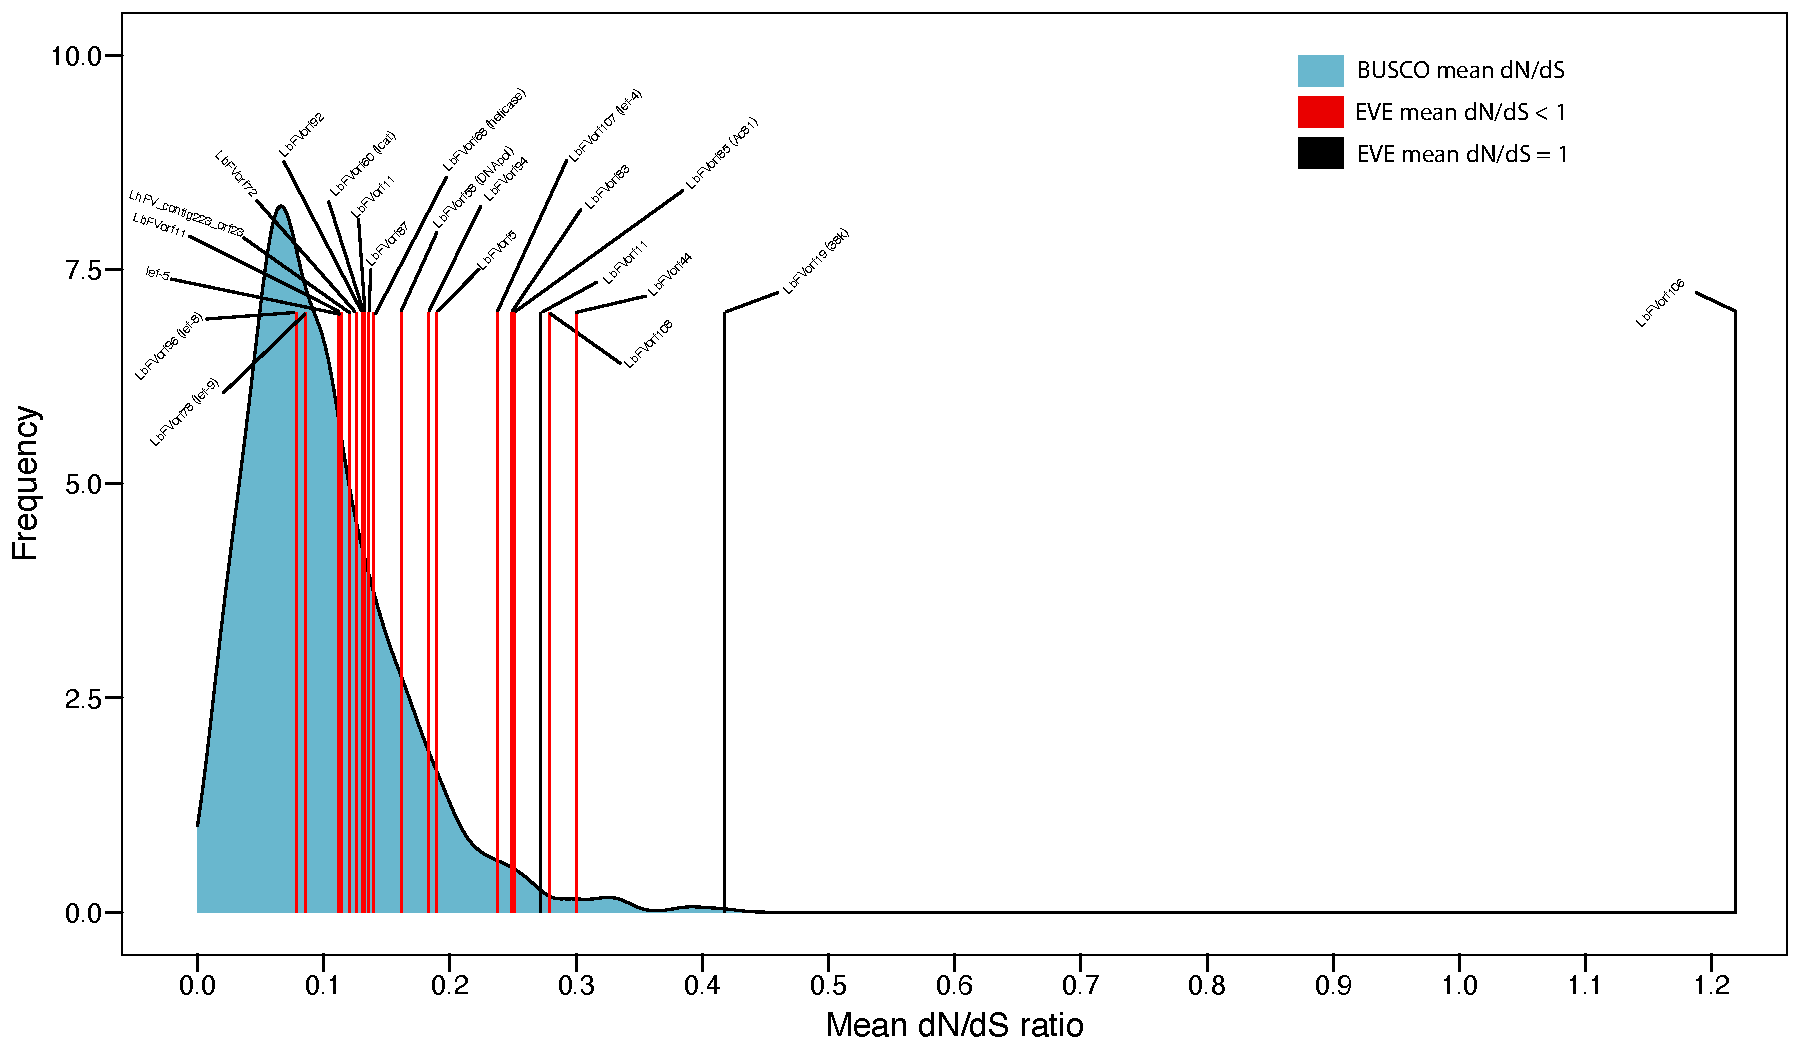
\includegraphics[width=\linewidth,height=\textheight,keepaspectratio]{dNdS_density_plot.pdf}\centering
\label{figure:dNdS_density_plot}
\caption[Paper3:Eucoilini filamentous EVE dN/dS mean distribution]{\textbf{Virally derived genes are under strong purifying selection in Eucoilini wasp genomes}. \textit{dN/dS} ratio for a set of 1000 universal arthropod genes (blue density curve) and for 18 virally derived genes found in \textit{Leptopilina}, \textit{Trybliographa}, \textit{Thrichoplasta} and \textit{Rhoptromeris} species (indicated by the red lines). Red lines indicate \textit{dN/dS} significantly below 1 while black lines indicate \textit{dN/dS} =1. The labels above the lines indicate the number of the ORF within the LbFV genome and the putative protein names are indicated between parenthesis.}
\end{figure}



\begin{figure}[!htpbt]
\includegraphics[width=\linewidth,height=\textheight,keepaspectratio]{PhD-master/figures/dNdS_position_plot.pdf}\centering
\caption[Paper3:Eucoilini filamentous EVE dN/dS distribution per site]{\textbf{\textit{dN/dS} profile along filamentous endogenous elements sites}. Line graph reporting \textit{dN/dS} values estimated for each codon position of the endogenous filamentous viral elements using FEL method. Sites detected to be under statistically significant positive or negative selection are reported as green point and red point  respectively (pvalue$<$0.05), while sites with the default FEL threshold pvalue (pvalue$<$0.1) are reported as black points.}
\label{figure:dNdS_position_plot}
\end{figure}


%\usepackage{pdflscape}

\begin{landscape}
\begin{table}
\caption[Paper3:HHpred and HHmmer result on Eucoilini filamentous EVEs]{\textbf{Homology search for the 25 filamentous proteins endogenized in Cynipid wasps}. A HHpred on PDB\_mmCIF70\_12\_Aug and a HHmer on alphafold\_uniprot\_Aug\_2022 databases were ran on all the 25 cluster AA alignments (HHpred and HHmer column results have the -HHpred and -HHmer names respectively). These analyses were done using the MPI toolkits \citep{zimmermann_completely_2018}.}
\tiny
\centering
\resizebox{\linewidth}{!}{%
\begin{tabular}{>{\hspace{0pt}}m{0.09\linewidth}|>{\hspace{0pt}}m{0.05\linewidth}>{\hspace{0pt}}m{0.058\linewidth}>{\hspace{0pt}}m{0.088\linewidth}>{\hspace{0pt}}m{0.054\linewidth}>{\hspace{0pt}}m{0.048\linewidth}>{\hspace{0pt}}m{0.048\linewidth}>{\hspace{0pt}}m{0.123\linewidth}>{\hspace{0pt}}m{0.054\linewidth}>{\hspace{0pt}}m{0.052\linewidth}>{\hspace{0pt}}m{0.058\linewidth}>{\hspace{0pt}}m{0.088\linewidth}>{\hspace{0pt}}m{0.054\linewidth}>{\hspace{0pt}}m{0.056\linewidth}} 
\toprule
Fonction/activity (by similarity) & Cluster\_name & ORF\_name & Prot\_name & Filamentous core & Eucoilini core & ID-HHpred & Name-HHpred & E-value-HHpred & Score\_HHpred & ID-HMMER & Name-HMMER & E-value-HMMER & Bitscore-HMMER \\ 
\cline{2-14}
\multirow{4}{*}{transcription/RNA polymerase} & Cluster115 & LbFVorf107 & Lef-4 & + & + &  &  &  &  & A0A0U1ZIV8-F1 & Lef-4 & 2.00E-117 & 404.5 \\
 & Cluster559 & LbFV\_orf038rc & Lef-5 & + & + & 6RUI\_I & DNA-directed RNA polymerase I subunit RPA12; RNA Polymerase I & 0.027 & 34.94 & A0A1D3TG76-F1 & Ribosome maturation factor RimM & 1.2e-23 & 38.9 \\
 & Cluster1614 & LbFVorf96 & Lef-8 & + & + & 4QIW\_B & DNA-directed RNA polymerase & 9.1e-10 & 140.24 & B9W484-F1 & DNA-directed RNA polymerase & 5.7e-240 & 810.2 \\
 & Cluster15 & LbFVorf78 & Lef-9 & + & + & 4QIW\_A & DNA-directed RNA polymerase & 2.00E-09 & 127.92 & A0A4Y2I2C6-F1 & DNA-directed RNA polymerase & 8.1e-23 & 91.1 \\ 
\cline{1-1}
\multirow{4}{*}{DNA replication/processing} & Cluster59 & LbFVorf68 & Helicase & + & + & 7BIL\_A & PIF1 helicase & 6.5e-10 & 118.77 & A0A0L7QZN7-F1 & ResIII domain-containing protein & 1.4e-50 & 182.9 \\
 & Cluster126 & LbFVorf58 & DNApol & + & + & 7KC0\_A & DNA polymerase & 4.8e-19 & 216.57 & A0A6C0AHJ6-F1 & DNA-directed DNA polymerasz & 9.00E-45 & 85.2 \\
 & Cluster2683 & LbFVorf92 & Primase/helicase & + & + & 7OM0\_B & DNA primase; Helicase & 4.1e-10 & 145.63 & A0A0U1ZLA9-F1 & Helicase & 9.2e-263 & 886.4 \\
 & Cluster22 & LbFVorf2 & Integrase & + &  & 1A0P\_A & Recombinase & 4.6e-10 & 93.03 &  &  &  &  \\ 
\cline{1-1}
JmjC Multigenic family & Cluster114 & LbFVorf11/13 & JmJC & + & + & 6F5R\_A & Lysine-specific demethylase 4D & 8.1e-19 & 144.01 & A0A6J1RRU0-F1 & Zinc finger protein & 7.7e-56 & 30.3 \\ 
\cline{1-1}
\multirow{2}{*}{Lipid} & Cluster1472 & PcFV\_scf2882\_orf4 & Mucin-like (lipid transport) &  &  & 1AV1\_A & Apolipoprotein A-I & 0.0034 & 45.88 &  &  &  &  \\
 & Cluster440 & LbFVorf60 & LCAT (inflammation regulation) & + & + & 4R1D\_A & Lipase, Hydrolase & 2.6e-13 & 139.08 & A0A1F7HJ92-F1 & AB hydrolase-1 domain-containing protein & 1.6e-264 & 891.7 \\ 
\cline{1-1}
\multirow{2}{*}{Host interaction} & Cluster965 & LbFVorf85 & Ac81 (nucleocapsid envelopment) & + & + &  &  &  &  & A0A0U1ZKX8-F1 & Ac81-like.1 & 7.9e-40 & 150 \\
 & Cluster45 & LbFVorf106 & OdV-E66 (ODV envelope component) & + & + & 3VSN\_A & Occlusion-derived virus envelope protein E66 & 6.2e-43 & 402.44 & B9W4B3-F1 & Putative envelope protein ODV-E66 & 5.4e-195 & 661 \\ 
\cline{1-1}
Structure/Capsid component, Phosphatase & Cluster38 & LbFVorf19 & 38k & + &  & 4XPZ\_A & RNA polymerase II subunit A C-terminal domain phosphatase & 2.1e-7 & 88.58 & B9W486-F1 & Putative 38K protein & 1.1e-79 & 279.8 \\ 
\cline{1-1}
\multirow{2}{*}{Unknown} & Cluster1692 & LbFVorf10 & None &  &  & 2K9H\_A & Hantavirus, Glycoprotein, Zinc Finger & 9.5e-7 & 54.68 &  &  &  &  \\
 & Cluster2164 & LbFVorf105 & None &  &  & 6H3A\_A & Transcription intermediary factor 1-beta & 0.0026 & 43.81 & A0A1A9UYJ1-F1 & F-box domain & 1.4e-50 & 185.5 \\
\bottomrule
\label{table:ORF_functions}
\end{tabular}
}
\end{table}

\end{landscape}

\begin{figure}[!htpbt]
\includegraphics[width=\linewidth,height=\textheight,keepaspectratio]{PhD-master/figures/Host_virus_phylogeny_last.pdf}\centering
\caption[Paper3:Recapitulastion of \textit{Naldaviricetes} EVEs in insects ]{\textbf{Summary of endogenized and domesticated viral elements of dsDNA viruses in arthropods}. \textbf{A} - Phylogeny of viruses of the class \textit{Naldaviricetes}, with the virus clades involved in endogenisation phenomena coloured. \textbf{B} - Phylogeny of insects including Hymenoptera and Hemiptera having integrated and/or domesticated genetic material from viruses of the class \textit{Naldaviricetes}. Event (1) corresponds to the domestication event of a betanudivirus in the common ancestor of Microgastroids, about 100 million years ago, which allows the production of PDVs \citep{bezier_polydnaviruses_2009}. Event (2) corresponds to the domestication of an unknown virus in the ancestor of at least two species of the Banchinae family which is independent of event (3) in which another unknown virus was domesticated in species of the Campopleginae family. Both allow the production of PDVs \citep{beliveau_genomic_2015,burke_presence_2021,legeai_genomic_2020}. Event (4) corresponds to a domestication event of a betanudivirus that took place about 20 million years ago and is found in the genome of \textit{V.canescens} and allows the production of VLPs \citep{pichon_recurrent_2015}. Event (5) corresponds to a domestication event of a betanudivirus that took place in the genome of \textit{F.arisanus} and allows the production of VLPs \citep{burke_rapid_2018}. Event (6) corresponds to a domestication event of a Filamentoviridae close to LhFV that occurred around 75 million years ago in part of the Eucoilini species described in the present paper, allowing the production of VLPs at least in \textit{L.boulardi} and \textit{T.rapae}. Another independent event involving a filamentous virus close to LbFV also occurred within the \textit{Rhoptromeris} genus. Event (7) corresponds to the endogenization and probably domestication of a Filamentoviridae closely related to PoFV that occurred recently within the \textit{P.orseoliae} genome (\hyperref[sec:chap1]{chapitre 1}:\textit{in review}). All the other unnumbered events correspond to independent \textit{a priori} events that show no trace of domestication.}
\label{figure:Host_virus_phylogeny_last}
\end{figure}


